\chapter{Fibrations and product-type operators}\label{ch:product}
\providecommand{\RelC}[2]{{}^{#1}\overline{#2}}
\providecommand{\Psipt}[1]{\Psi^{#1}_{\phi\text{-}\mathrm{pt}}}
\providecommand{\Dfm}{\operatorname{Dfm}}
\providecommand{\fib}{\mathrm{fib}}
\providecommand{\Sigmapt}[1]{\Sigma^{#1}_{\phi}}

Many problems in index theory involve two kinds of operators at once: operators
acting along the fibres of a fibration, and operators acting on its total space.
The proof of the index theorem in \cref{ch:families} deforms an operator built
from both kinds, and needs a single algebra in which such deformations make sense.
Neither the ordinary pseudodifferential operators on $M$ nor the fibrewise
families are large enough. This chapter builds the algebra and its two symbols.

The families version of the Atiyah--Singer index theorem concerns elliptic
operators on the fibres of a fibration $\phi:M\longrightarrow B$; rather than a
family $A_b\in\Psido m(Z;E,F)$ simply parametrized by $b\in B$, the manifold on
which $A_b$ acts is allowed to be `twisted' by diffeomorphisms of the fibre $Z$
as $b$ varies. This chapter sets up the analytic machinery needed for that
theorem and for the index formulae of \cref{ch:families} and \cref{ch:eta}.

In the first three sections we define fibrations, the space
$\Psido m(M/B;E,F)$ of pseudodifferential operators acting on the fibres, and
the index bundle $\ind_a(A)\in K^0(B)$ of an elliptic family. The rest of the
chapter constructs a larger algebra, the \emph{product-type} pseudodifferential
operators $\Psipt{m,m'}(M;E,F)$, which contains both the classical
pseudodifferential operators on the total space $M$ and the classical fibrewise
families.
Their kernels are conormal, in a `product' sense, to the nested pair of
submanifolds $\Diag_M\subset M^2_\phi\subset M^2$, where $M^2_\phi$ is the fibre
product. Following the pattern of \cref{ch:conormal}, these kernels are
defined as inverse Fourier transforms of symbols, now smooth (up to weights) on a
compactification of a vector space $W$ relative to a subspace $V$; this
\emph{relative compactification} turns out to be a product of two radial
compactifications. A product-type operator has two symbols: the usual principal
symbol, defined on a blown-up cosphere bundle, and a \emph{base symbol}, which is
a family of pseudodifferential operators on the fibres parametrized by
$T^*B\setminus0$. If both are invertible the operator is \emph{fully elliptic},
has a parametrix modulo smoothing operators, and is Fredholm.

We use freely the radial compactification of a vector space
(\cref{ch:distributions}), conormal distributions and their symbols
(\cref{ch:conormal}), pseudodifferential operators on compact manifolds and
their Fredholm properties (\cref{ch:manifolds}), and the elementary $K$-theory
of \cref{ch:index} and \cref{ch:bott}. All manifolds are without boundary unless
otherwise stated, and all vector bundles are complex.

\emph{Symbol conventions.} As in \cref{ch:euclidean,ch:manifolds}, $\Psido m$ and
$\Ic m$ denote the general spaces, defined by symbol estimates, and
$\Psido m_{\mathrm{ph}}$, $\Ic m_{\mathrm{ph}}$ the classical (one-step
polyhomogeneous) subspaces. The fibrewise families of
\cref{product:sec:families,product:sec:index-bundle} are treated in the general
class, the homogeneous principal symbol being available only for the classical
subclass. The product-type calculus of
\cref{product:sec:symbols,product:sec:conormal,product:sec:operators} is built from
\emph{weighted smooth} symbols on the relative compactification, so it is a
classical calculus: it contains the classical ordinary and fibrewise operators, but
not the general ones (\cref{product:rem:nonclassical}). Classical spaces of real
order are nested only under integer shifts of the order:
$\Psido m_{\mathrm{ph}}\subset\Psido{m+j}_{\mathrm{ph}}$ for $j\in\N_0$, but for
instance $\Id\notin\Psido{1/2}_{\mathrm{ph}}$; the same holds, in each of the two
orders, for the product-type spaces.

\section{Fibrations}\label{product:sec:fibrations}

\begin{definition}\label{product:def:fibration}
A \emph{fibration} (of compact manifolds) is a smooth surjective map
$\phi:M\longrightarrow B$ between compact manifolds which is a
\emph{submersion}, i.e.\ $\phi_*:T_mM\longrightarrow T_{\phi(m)}B$ is surjective
for every $m\in M$. The \emph{fibre} over $b\in B$ is $Z_b=\phi^{-1}(b)$
(\cref{product:fig:fibration}). We
indicate a fibration by the diagram $Z\text{---}M\overset{\phi}{\longrightarrow}B$,
where $Z$ is the typical fibre (see below).
\end{definition}

If $M$ is compact, $B$ is connected and $\phi$ is a submersion, then $\phi$ is
automatically surjective (if $M\neq\emptyset$): its range is open, since $\phi$ is
a submersion, and closed, since $M$ is compact.

For maps between manifolds with corners, such as those between the blown-up spaces used
later in this chapter, a surjective submersion need not be a fibration; the appropriate
replacement is the notion of a b-fibration (\cref{blowup:def:bfib}, see
\cref{blowup:sec:bfib}).

\begin{theorem}[Local triviality]\label{product:thm:local-triviality}
Let $\phi:M\longrightarrow B$ be a fibration.
\begin{enumerate}[label=\textup{(\arabic*)}]
\item Each fibre $Z_b$ is a compact embedded submanifold of $M$ of dimension
$\dim M-\dim B$; the fibres over each connected component of $B$ are all
diffeomorphic, so if $B$ is connected all fibres are diffeomorphic to a fixed
compact manifold $Z$.
\item Each $b\in B$ has an open neighbourhood $U_b$ with a diffeomorphism
$f_b:\phi^{-1}(U_b)\longrightarrow Z_b\times U_b$ such that
$\pi_{U}\circ f_b=\phi$, where $\pi_U:Z_b\times U_b\longrightarrow U_b$ is the
projection. If $B$ is connected, $Z_b$ may be replaced by the fixed fibre $Z$.
\item Suppose $B$ is connected \textup{(}in general, apply this on each component,
with the fibre $Z$ of that component\textup{)}. For two trivializations as in
\textup{(2)} with values in $Z\times U_b$, $Z\times U_{b'}$, $f_{b'}\circ f_b^{-1}$
is a diffeomorphism of $Z\times(U_b\cap U_{b'})$ of the form $(z,c)\longmapsto(f_{b'b}(c)(z),c)$ where
$f_{b'b}:U_b\cap U_{b'}\longrightarrow\Dfm(Z)$ is a smooth family of
diffeomorphisms of $Z$ \textup{(}meaning that $(z,c)\mapsto f_{b'b}(c)(z)$ is
smooth\textup{)}, and the cocycle condition
$f_{b''b'}f_{b'b}=f_{b''b}$ holds on $U_b\cap U_{b'}\cap U_{b''}$.
\end{enumerate}
\end{theorem}

\begin{proof}
If $t_1,\dots,t_p$ are local coordinates on $B$ centred at $b$, the functions
$\phi^*t_i$ have linearly independent differentials at each point of $Z_b$
because $\phi$ is a submersion, so by the implicit function theorem
$Z_b=\{\phi^*t_1=\dots=\phi^*t_p=0\}$ is an embedded submanifold of codimension
$p=\dim B$; it is compact, being closed in $M$.

Choose a Riemannian metric on $M$ and let $H_m\subset T_mM$ be the orthogonal
complement of $\ker\phi_*=T_mZ_{\phi(m)}$. Then $\phi_*:H_m\longrightarrow
T_{\phi(m)}B$ is an isomorphism and depends smoothly on $m$, so each vector field
$v$ on an open set $U\subset B$ has a unique smooth `horizontal lift' $\tilde v$ to
$\phi^{-1}(U)$, with $\tilde v(m)\in H_m$ and $\phi_*\tilde v=v$. Let $U_b$ be a
coordinate ball, $\{|t|<r\}$, centred at $b$. For $c\in U_b$ with coordinates
$t(c)$ consider the constant-coefficient vector field
$v_c=\sum_it_i(c)\pa_{t_i}$ and its horizontal lift $\tilde v_c$. The integral
curve of $v_c$ starting at $b$ is $s\mapsto st(c)$, which stays in the compact set
$\{|t|\le|t(c)|\}\subset U_b$ for $s\in[0,1]$; hence the integral curves of
$\tilde v_c$ starting on $Z_b$ stay in the compact set $\phi^{-1}(\{|t|\le
|t(c)|\})$ and exist up to time $1$. Let $F(z,c)=\exp(\tilde v_c)(z)$ be the
time-one flow. By smooth dependence of solutions of ordinary differential
equations on parameters, $F:Z_b\times U_b\longrightarrow\phi^{-1}(U_b)$ is smooth,
and $\phi(F(z,c))=c$. It is a bijection with smooth inverse
$m\longmapsto(\exp(-\tilde v_{\phi(m)})(m),\phi(m))$, so $f_b=F^{-1}$ is a
diffeomorphism as in (2). In particular the fibres
over $U_b$ are all diffeomorphic to $Z_b$, so the set of
$c\in B$ with $Z_c$ diffeomorphic to a given fibre is open and closed; this
proves (1), and (2) with a fixed $Z$ when $B$ is connected (composing $f_b$ with
a diffeomorphism $Z_b\cong Z$). Without connectedness the fibre type may change
between components: for $B$ two points, one fibre may be a circle and the other
two circles. Part (3) is immediate from (2): $f_{b'}\circ
f_b^{-1}$ commutes with the projections to $U_b\cap U_{b'}$, so has the stated
form, and the cocycle condition is just associativity of composition.
\end{proof}

\begin{figure}[ht]
\centering
\begin{tikzpicture}[>=Stealth]
\fill[gray!12] (2.2,0.95) rectangle (3.8,3.05);
\draw[thick] plot[smooth] coordinates {(0,3.0) (1.5,3.2) (3,2.9) (4.5,3.15) (6,3.0)};
\draw[thick] plot[smooth] coordinates {(0,1.0) (1.5,0.8) (3,1.1) (4.5,0.85) (6,1.0)};
\foreach \x/\yt/\yb in {0/3.0/1.0, 0.75/3.12/0.88, 1.5/3.2/0.8, 2.25/3.05/0.95,
  3.75/3.02/0.97, 4.5/3.15/0.85, 5.25/3.07/0.93, 6/3.0/1.0}{
  \draw[gray] (\x,\yb) .. controls (\x+0.25,{(\yt+\yb)/2-0.5}) and
    (\x-0.25,{(\yt+\yb)/2+0.5}) .. (\x,\yt);}
\draw[very thick] (3,1.1) .. controls (3.3,1.5) and (2.7,2.5) .. (3,2.9);
\node[right,font=\small] at (3.05,2.1) {$Z_b$};
\node[font=\small] at (6.5,2.1) {$M$};
\draw[thick] (0,-0.3)--(6,-0.3);
\node[font=\small] at (6.5,-0.3) {$B$};
\fill (3,-0.3) circle (1.8pt) node[below,font=\small]{$b$};
\draw[decorate,decoration={brace,mirror,amplitude=4pt}] (2.2,-0.55)--(3.8,-0.55)
  node[midway,below=5pt,font=\footnotesize]{$U_b$};
\draw[->] (-0.5,2.0)--node[left,font=\small]{$\phi$}(-0.5,-0.2);
\draw[densely dashed] (3,0.95)--(3,-0.25);
\node[font=\footnotesize,align=left,anchor=west] at (7.1,2.1)
  {shaded: $\phi^{-1}(U_b)\cong Z\times U_b$};
\end{tikzpicture}
\caption{A fibration $\phi:M\to B$ over a connected base. Each fibre
$Z_b=\phi^{-1}(b)$ is a compact manifold diffeomorphic to a fixed $Z$, and over a
small open set $U_b$ the total space is a product $Z\times U_b$
(\cref{product:thm:local-triviality}; over a disconnected base the fibre type is
fixed on each component). Globally the fibres may
be glued together by diffeomorphisms, so $M$ need not be $Z\times B$.}
\label{product:fig:fibration}
\end{figure}

Conversely, $M$ is recovered from the trivializations and the transition maps
$f_{b'b}$; thus a fibration is a fibre bundle with fibre $Z$ and structure group
$\Dfm(Z)$. If the transition maps can be chosen to take values in a subgroup
$G\subset\Dfm(Z)$, the structure group is said to be \emph{reduced} to $G$.

\begin{proposition}[Pull-back]\label{product:prop:pullback}
Let $\phi:M\longrightarrow B$ be a fibration and $F:\tilde B\longrightarrow B$ a
smooth map from a compact manifold. Then
$\tilde M=\{(m,\tilde b)\in M\times\tilde B;\phi(m)=F(\tilde b)\}$ is an embedded
submanifold of $M\times\tilde B$ and $\tilde\phi:\tilde M\longrightarrow\tilde
B$, $\tilde\phi(m,\tilde b)=\tilde b$, is a fibration with fibre
$\tilde\phi^{-1}(\tilde b)=Z_{F(\tilde b)}$.
\end{proposition}

\begin{proof}
$\tilde M$ is the preimage of $\Diag_B$ under $\Phi=\phi\times
F:M\times\tilde B\longrightarrow B\times B$. Since $\phi$ is a submersion, the
range of $\Phi_*$ contains $TB\times\{0\}$, and $TB\times\{0\}$ together with
$T\Diag_B$ spans $T(B\times B)$; so $\Phi$ is transversal to $\Diag_B$ and
$\tilde M$ is an embedded submanifold of codimension $\dim B$, compact since it
is closed. Its tangent space is $\{(v,w);\phi_*v=F_*w\}$; given $w\in
T_{\tilde b}\tilde B$ we can solve $\phi_*v=F_*w$, so $\tilde\phi$ is a
submersion, and it is surjective because $F$ is defined on all of $\tilde B$ and
$\phi$ is surjective.
\end{proof}

\begin{proposition}[Composites and products]\label{product:prop:composite}
If $\phi':M'\longrightarrow M$ and $\phi:M\longrightarrow B$ are fibrations then
$\phi\circ\phi':M'\longrightarrow B$ is a fibration; its fibre over $b$ is
$(\phi')^{-1}(Z_b)$, which is itself the total space of the fibration
$\phi'|:(\phi')^{-1}(Z_b)\longrightarrow Z_b$ obtained by restriction.
If $\phi_i:M_i\longrightarrow B_i$, $i=1,2$, are fibrations then so is
$\phi_1\times\phi_2:M_1\times M_2\longrightarrow B_1\times B_2$.
\end{proposition}

\begin{proof}
Composites and products of surjective submersions are surjective submersions.
The restriction of $\phi'$ to $(\phi')^{-1}(Z_b)$ is the pull-back of $\phi'$
under the inclusion $Z_b\hookrightarrow M$, so is a fibration by
\cref{product:prop:pullback}.
\end{proof}

Note that the fibre of $\phi\circ\phi'$ need not be diffeomorphic to the product
$Z\times Z'$ of the fibres; it is in general a non-trivial fibration over $Z$.

\subsection{Vertical bundles and connections}
The \emph{vertical tangent bundle} $T(M/B)\subset TM$ is the null bundle of
$\phi_*$, so $T_m(M/B)=T_mZ_{\phi(m)}$, and there are short exact sequences of
vector bundles over $M$
\begin{equation}\label{product:eq:vertical}
0\longrightarrow T(M/B)\longrightarrow TM\overset{\phi_*}\longrightarrow\phi^*TB
\longrightarrow0,\qquad
0\longrightarrow\phi^*T^*B\overset{\phi^*}\longrightarrow T^*M\longrightarrow
T^*(M/B)\longrightarrow0,
\end{equation}
where $T^*(M/B)$ is the dual of $T(M/B)$. The second sequence identifies
$\phi^*T^*B$ with the subbundle of covectors annihilating the fibres. We denote
by $S^*(M/B)$ and $\phi^*S^*B$ the corresponding sphere bundles (quotients of the
complements of the zero sections by $\R_+$).

\begin{definition}\label{product:def:connection}
A \emph{connection} on the fibration $\phi$ is a choice of a smooth subbundle
$H\subset TM$ complementary to $T(M/B)$. Then $\phi_*:H\longrightarrow\phi^*TB$ is
an isomorphism, so a connection is the same as a splitting of the first sequence
in \eqref{product:eq:vertical}, and dually of the second.
\end{definition}

The proof of \cref{product:thm:local-triviality} used the connection given by
the orthogonal complement for a Riemannian metric, so connections always exist.

The \emph{fibre density bundle} $\Omega(M/B)=\Omega(T(M/B))$ is the bundle of
densities on the fibres. From \eqref{product:eq:vertical} there is a canonical
isomorphism $\Omega(M)\cong\Omega(M/B)\otimes\phi^*\Omega(B)$; in particular
a smooth positive section of $\Omega(M/B)$ restricts to a smooth positive density
on each fibre.

\subsection{The fibre product}
Applying \cref{product:prop:pullback} with $F=\phi$ gives the \emph{fibre
product}
\begin{equation*}
M^2_\phi=M\times_\phi M=\{(m,m')\in M^2;\phi(m)=\phi(m')\},
\end{equation*}
an embedded submanifold of $M^2$ of codimension $b=\dim B$. It fibres over $M$
(by either projection) with fibre $Z$, and over $B$ with fibre $Z^2$. It contains
the diagonal, so we have a nested pair of embedded submanifolds
\begin{equation}\label{product:eq:nested}
\Diag_M\subset M^2_\phi\subset M^2.
\end{equation}
If $(z,y)$ are local coordinates on $M$ in which $\phi(z,y)=y$ (\emph{fibred
coordinates}), and $(z',y')$ is a second copy, then near a point of $M^2_\phi$
\begin{equation}\label{product:eq:nested-coords}
\Diag_M=\{z=z',\ y=y'\}\subset M^2_\phi=\{y=y'\}\subset M^2.
\end{equation}
We write $\pi_L,\pi_R:M^2\longrightarrow M$ for the projections and also for
their restrictions to $M^2_\phi$, and set
$\Omega_R=\pi_R^*\Omega(M/B)$ over $M^2_\phi$; for bundles $E$, $F$ over $M$ we
write $\Hom(E,F)=\pi_L^*F\otimes\pi_R^*E^*$ over $M^2$ or $M^2_\phi$.

\begin{lemma}\label{product:lem:conormal-identifications}
For a fibration $\phi:M\longrightarrow B$:
\begin{enumerate}[label=\textup{(\roman*)}]
\item the conormal bundle of the fibre diagonal is
$N^*_{(m,m')}M^2_\phi=\{(\phi^*\eta,-\phi^*\eta);\eta\in T^*_{\phi(m)}B\}$, so
$N^*M^2_\phi\cong(\phi\circ\pi_L)^*T^*B$ and its sphere bundle is the fibre
product $SN^*M^2_\phi\cong M^2_\phi\times_BS^*B$, which is the fibre product
of the pulled-back fibration $\pi^*M=M\times_BS^*B\longrightarrow S^*B$,
$\pi:S^*B\longrightarrow B$;
\item $N^*\Diag_M\cong T^*M$, by $(\xi,-\xi)\longmapsto\xi$;
\item under \textup{(ii)}, the restriction $N^*M^2_\phi|_{\Diag_M}$ is
identified with $\phi^*T^*B\subset T^*M$, and the quotient
\begin{equation*}
N^*\Diag_M/N^*M^2_\phi|_{\Diag_M}
\end{equation*}
with $T^*(M/B)$, the conormal bundle of $\Diag_M$ as a submanifold of
$M^2_\phi$.
\end{enumerate}
\end{lemma}

\begin{proof}
$M^2_\phi$ is the preimage of $\Diag_B$ under $\phi\times\phi$, a submersion, so
its conormal space at $(m,m')$ is the pull-back of $N^*\Diag_B=\{(\eta,-\eta)\}$.
This gives (i); the description of the sphere bundle follows. Part (ii) is
standard, and (iii) follows by comparing (i) and (ii) with
\eqref{product:eq:vertical}; in the coordinates \eqref{product:eq:nested-coords}
it says that $N^*M^2_\phi$ is spanned by the $dy_j-dy'_j$.
\end{proof}

\section{Families of pseudodifferential operators}\label{product:sec:families}

Throughout, $\phi:M\longrightarrow B$ is a fibration with typical fibre $Z$, and
we set $f=\dim Z$, $b=\dim B$. (If $B$ is disconnected, $Z$ and $f$ may depend on
the component; all statements are then componentwise.) One could define operators on the fibres by
patching together, using \cref{product:thm:local-triviality}, smooth families of
operators on $Z$, relying on the invariance of pseudodifferential operators under
diffeomorphisms. It is more direct to use conormal distributions on the fibre
product. Recall from \cref{ch:conormal} and \cref{ch:manifolds} that
$\Psido m(X;E,F)=\Ic m(X^2,\Diag;\Hom(E,F)\otimes\Omega_R)$, with the order
normalization of \cref{ch:conormal} (for which a conormal distribution of order
$m$ at a submanifold of codimension $c$ in a manifold of dimension $n$ has a
symbol of order $m+\frac n4-\frac c2$).

\begin{definition}\label{product:def:fibre-psido}
The space of \emph{pseudodifferential operators on the fibres} of $\phi$, acting
from sections of $E$ to sections of $F$, is
\begin{equation*}
\Psido m(M/B;E,F)=\Ic{m-\frac b4}(M^2_\phi,\Diag_M;\Hom(E,F)\otimes\Omega_R).
\end{equation*}
The subspace of \emph{classical} families, $\Psido m_{\mathrm{ph}}(M/B;E,F)$, is
defined in the same way using $\Ic{m-\frac b4}_{\mathrm{ph}}$. An element acts on
$u\in\CI(M;E)$ by $Au=(\pi_L)_*(A\cdot\pi_R^*u)$, where now
$\pi_L,\pi_R:M^2_\phi\longrightarrow M$ and the push-forward is fibre integration
along the right factor, using the density factor $\Omega_R=\pi_R^*\Omega(M/B)$.
\end{definition}

The shift in order is such that the symbols have order $m$: $\dim M^2_\phi=2f+b$
and $\Diag_M$ has codimension $f$ in $M^2_\phi$, so the symbol order is
$m-\frac b4+\frac{2f+b}4-\frac f2=m$.

\begin{discussion}
  Why the fibre product? An operator acting on each fibre separately never moves
  information from one fibre to another, so its Schwartz kernel on $M^2$ vanishes
  unless the two points lie in the same fibre, i.e.\ it is supported in
  $M^2_\phi$. On $M^2_\phi$ it is an ordinary pseudodifferential kernel in the
  fibre variables, conormal to the diagonal. Viewed on $M^2$ it is a
  $\delta$-function in the base directions $y-y'$ times such a kernel; this
  picture is the starting point for the product-type calculus later in the
  chapter.
\end{discussion}

\begin{lemma}\label{product:lem:local-families}
Let $U\subset B$ be an open ball over which there is a trivialization
$\phi^{-1}(U)\cong Z\times U$ as in \cref{product:thm:local-triviality}, and
bundle isomorphisms $E|_{\phi^{-1}(U)}\cong\pi_Z^*E_0$,
$F|_{\phi^{-1}(U)}\cong\pi_Z^*F_0$ for bundles $E_0$, $F_0$ over $Z$ (these exist
since $U$ is contractible). Then restriction of kernels gives an identification
\begin{equation*}
\Psido m(M/B;E,F)\big|_U\cong\CI(U;\Psido m(Z;E_0,F_0)),
\end{equation*}
where $\Psido m(Z;E_0,F_0)$ carries its Fréchet topology and the right side
consists of the smooth maps into it; similarly
$\Psido m_{\mathrm{ph}}(M/B;E,F)|_U\cong\CI(U;\Psido m_{\mathrm{ph}}(Z;E_0,F_0))$.
\end{lemma}

\begin{proof}
Over $U$ the trivialization identifies $M^2_\phi$ with $Z^2\times U$, $\Diag_M$
with $\Diag_Z\times U$ and $\Omega_R$ with the right density bundle of $Z$. The
submanifold $\Diag_Z\times U$ is a product, the variables in $U$ being variables
along it, so by the definition of conormal distributions in local coordinates
(\cref{ch:conormal}) an element of $\Ic{m''}(Z^2\times U,\Diag_Z\times U)$ is
locally the inverse Fourier transform in the normal variables of a symbol
depending smoothly on the variables in $Z$ and $U$; that is, it is a smooth
family, parametrized by $U$, of elements of $\Ic{m''+\frac b4}(Z^2,\Diag_Z)$
(the shift by $\frac b4$ comes from the change of dimension). With
$m''=m-\frac b4$ this is $\CI(U;\Psido m(Z;E_0,F_0))$; the symbol is classical
in the normal variables if and only if each member of the family is.
\end{proof}

In particular $\Psido m(M/B;E,F)$ does not depend on choices, and its elements are
the families which are, locally in $B$, smooth families of pseudodifferential
operators on a fixed fibre, glued by the transition maps of
\cref{product:thm:local-triviality}(3).

Note that the elements of $\Psido m(M/B;E,F)$, as operators on $M$, have
Schwartz kernels supported in $M^2_\phi$, with a $\delta$-singularity in the
normal directions, whereas elements of $\Psido m(M;E,F)$ have kernels which are
smooth off the diagonal. For $\dim B>0$ the only operators in both spaces are
fibrewise differential operators (\cref{product:ex:intersection}).

\begin{proposition}\label{product:prop:families}
Let $\phi:M\longrightarrow B$ be a fibration and $E$, $F$, $G$ vector bundles
over $M$.
\begin{enumerate}[label=\textup{(\arabic*)}]
\item \textup{(Action)} Each $A\in\Psido m(M/B;E,F)$ defines a continuous linear
map $A:\CI(M;E)\longrightarrow\CI(M;F)$. It acts on the fibres: if
$u\in\CI(M;E)$ and $u|_{Z_b}=0$ then $Au|_{Z_b}=0$, so
\begin{equation*}
A_bv=(Au)|_{Z_b},\quad u\in\CI(M;E),\ u|_{Z_b}=v,
\end{equation*}
defines $A_b\in\Psido m(Z_b;E_b,F_b)$, where $E_b=E|_{Z_b}$. Moreover
$A(\phi^*\chi\,u)=\phi^*\chi\,Au$ for all $\chi\in\CI(B)$.
\item \textup{(Smoothing families)}
$\Psido{-\infty}(M/B;E,F)=\bigcap_m\Psido m(M/B;E,F)=\CI(M^2_\phi;\Hom(E,F)\otimes
\Omega_R)$.
\item \textup{(Symbol)} There is a principal symbol map giving a short exact
sequence
\begin{equation*}
\Psido{m-1}(M/B;E,F)\hookrightarrow\Psido m(M/B;E,F)\overset{\sigma_m}
\longrightarrow\Symq m(T^*(M/B);\hom(E,F)),
\end{equation*}
where $\Symq m=S^m/S^{m-1}$ is the quotient of the symbol spaces on the vector
bundle $T^*(M/B)\longrightarrow M$ (as in \cref{ch:manifolds}); $\sigma_m(A)$
restricts on $T^*Z_b$ to $\sigma_m(A_b)$. For classical families the principal
symbol has a homogeneous representative and there is a short exact sequence
\begin{equation*}
\Psido{m-1}_{\mathrm{ph}}(M/B;E,F)\hookrightarrow\Psido m_{\mathrm{ph}}(M/B;E,F)
\overset{\sigma_m}\longrightarrow\CI_{[m]}(T^*(M/B)\setminus0;\hom(E,F)),
\end{equation*}
where $\CI_{[m]}$ denotes smooth sections, homogeneous of degree $m$, of the
pull-back of $\hom(E,F)$ to $T^*(M/B)\setminus0$. (For a general family no
homogeneous representative need exist: a constant family of fibrewise multipliers
with local symbol $\sin(\log\ang\zeta)$ is of order $0$ but not classical.)
\item \textup{(Composition)} If $A\in\Psido m(M/B;F,G)$ and
$B'\in\Psido{m'}(M/B;E,F)$ then $AB'\in\Psido{m+m'}(M/B;E,G)$, $(AB')_b=A_bB'_b$
and $\sigma_{m+m'}(AB')=\sigma_m(A)\sigma_{m'}(B')$.
\item \textup{(Adjoints)} Given Hermitian metrics on $E$, $F$ and a positive fibre
density, the fibrewise adjoints $A_b^*$ form an element $A^*\in\Psido m(M/B;F,E)$,
with $\sigma_m(A^*)=\sigma_m(A)^*$.
\item \textup{(Asymptotic completeness)} If $A_j\in\Psido{m-j}(M/B;E,F)$
for $j\in\N_0$, then there exists an element $A\in\Psido m(M/B;E,F)$, unique
modulo $\Psido{-\infty}(M/B;E,F)$, such that
$A-\sum_{j<N}A_j\in\Psido{m-N}(M/B;E,F)$ for all $N$.
\end{enumerate}
Parts \textup{(1)}, \textup{(2)}, \textup{(4)}, \textup{(5)} and \textup{(6)} hold
equally for the classical families $\Psido\cdot_{\mathrm{ph}}(M/B)$.
\end{proposition}

\begin{proof}
All statements are local in $B$, since the kernels are supported in $M^2_\phi$.
Choose a finite cover of $B$ by balls $U_i$ as in \cref{product:lem:local-families}
and a partition of unity $\chi_i\in\CIc(U_i)$. Multiplication by $\phi^*\chi$,
$\chi\in\CI(B)$, commutes with $A$: by the definition of the action,
$A(\phi^*\chi\,u)=(\pi_L)_*\big(A\cdot\pi_R^*(\phi^*\chi)\,\pi_R^*u\big)$, and
$\pi_R^*\phi^*\chi=\pi_L^*\phi^*\chi$ as functions on $M^2_\phi$, since
$\phi\circ\pi_L=\phi\circ\pi_R$ there; so the factor comes out of the
push-forward along the right factor. (The support of the kernel alone would not
suffice: a derivative of $\delta(y-y')$ has the same support but does not commute
with $\phi^*\chi$; it is excluded because $A$ is a distribution on $M^2_\phi$, not
on $M^2$.) So $A=\sum_i\phi^*\chi_i\,A$ and each term is,
by \cref{product:lem:local-families}, a smooth family over $U_i$ of
pseudodifferential operators on $Z$, with compact support in $U_i$.

Every construction of the calculus on the compact manifold $Z$ is continuous
in the Fréchet topologies involved: the action $\Psido m(Z)\times\CI(Z)
\longrightarrow\CI(Z)$, composition, the symbol map, adjoints, and the
quantization of symbols. Hence each of them maps smooth families to smooth
families, and (1), (3), (4), (5) follow from the corresponding statements for
a single compact manifold in \cref{ch:manifolds} (and the classical statements
from the classical calculus there). For (1) note also that a smooth
family $u\in\CI(U\times Z;E_0)$ is mapped to a smooth family, i.e.\ to an element
of $\CI(U\times Z;F_0)$. In (3) the principal symbols of the local families
(classes modulo $S^{m-1}$, respectively homogeneous functions in the classical
case) patch together because the principal symbol is invariant under the
diffeomorphisms $f_{b'b}(c)$, and its restriction to $T^*Z_b$ is the symbol of
$A_b$; the null space of $\sigma_m$ is $\Psido{m-1}(M/B)$, respectively
$\Psido{m-1}_{\mathrm{ph}}(M/B)$, by the corresponding property of conormal
distributions, and surjectivity follows by quantizing $\chi_i\sigma$ in each $U_i$
and summing. Part (2) is the definition of
conormal distributions of order $-\infty$, and (6) follows from asymptotic
completeness of conormal distributions on $M^2_\phi$ (or locally from the
parameter version of Borel's lemma) together with the partition of unity.
\end{proof}

\begin{definition}\label{product:def:family-elliptic}
$A\in\Psido m(M/B;E,F)$ is \emph{elliptic} if a representative $a$ of
$\sigma_m(A)$ is invertible for $|\zeta|\ge R$, with $|a^{-1}|\le C\ang\zeta^{-m}$
there (for some metric on $T^*(M/B)$ and constants $R$, $C$), as in
\cref{manifolds:def:elliptic,manifolds:lem:elliptic}; for classical $A$ this means
that the homogeneous principal symbol is invertible at each point of
$T^*(M/B)\setminus0$. Equivalently each $A_b$ is elliptic: the constants for $A_b$
can be chosen locally uniformly in $b$, since $|a(b',\zeta)-a(b,\zeta)|\le
C|b-b'|\ang\zeta^m$ in a local trivialization, and $B$ is compact.
\end{definition}

\begin{proposition}\label{product:prop:family-parametrix}
If $A\in\Psido m(M/B;E,F)$ is elliptic there exists $Q\in\Psido{-m}(M/B;F,E)$
with
\begin{equation*}
QA-\Id_E\in\Psido{-\infty}(M/B;E),\qquad AQ-\Id_F\in\Psido{-\infty}(M/B;F).
\end{equation*}
\end{proposition}

\begin{proof}
Over each $U_i$ as above, $A$ is a smooth family of elliptic operators on $Z$.
The construction of a parametrix in \cref{ch:manifolds} --- quantize the inverse
of the principal symbol to get $Q_0$ with $Q_0A=\Id-R$, $R$ of order $-1$, then
take $Q\sim\sum_jR^jQ_0$ --- uses only operations continuous in the
Fréchet topologies together with asymptotic summation, which can be carried out
with smooth dependence on parameters (and which stays in the classical calculus if
$A$ is classical, \cref{manifolds:thm:parametrix}). So there are
$Q_i\in\CI(U_i;\Psido{-m}(Z))$
with $Q_iA-\Id$ and $AQ_i-\Id$ smoothing families over $U_i$. Set
$Q=\sum_i\phi^*\chi_i\,Q_i\in\Psido{-m}(M/B;F,E)$. Since multiplication by
$\phi^*\chi_i$ commutes with fibre operators,
\begin{gather*}
QA=\sum_i\phi^*\chi_i\,Q_iA=\Id_E-\sum_i\phi^*\chi_i(\Id-Q_iA),\\
AQ=\sum_i\phi^*\chi_i\,AQ_i=\Id_F-\sum_i\phi^*\chi_i(\Id-AQ_i),
\end{gather*}
and the error terms are smoothing families. If $A$ is classical, so is $Q$.
\end{proof}

Unlike the case of a single operator, the partition of unity on $B$ introduces
no error at all, because it commutes with the operators. The errors could also
be improved directly: if $Q_0A=\Id-R$ with $R\in\Psido{-1}(M/B;E)$, the Neumann
series $\sum_jR^jQ_0$ is asymptotically summable by
\cref{product:prop:families}(6).

\section{The index bundle}\label{product:sec:index-bundle}

We now associate to an elliptic family $A\in\Psido m(M/B;E,F)$ an element of
$K^0(B)$ generalizing the index of a single elliptic operator. The null spaces
$\Nul(A_b)$ need not have constant dimension, so need not form a vector bundle;
following \cite{Atiyah-Singer-IV} we first stabilize the family by a finite rank
perturbation so that it becomes surjective.

\begin{question}
  Why not define the index bundle as $[\Nul A]-[\Nul A^*]$ directly?
\end{question}
\begin{answer}
  Because $\dim\Nul A_b$ can jump. For the elliptic family
  $A_b=D_\theta+b$ on the circle, $b\in[-\frac12,\frac12]$, the eigenvalues are
  $k+b$, $k\in\Z$, so the null space is the constants at $b=0$ and zero
  elsewhere; the same happens for $A_b^*=A_b$. Only the difference $\dim\Nul A_b-\dim\Nul A_b^*$ is stable. Adding $N$ fixed
  sections makes every $\tilde A_b$ surjective, so the cokernel vanishes and the
  null spaces have the constant dimension $N+\ind A_b$. This is the same idea as
  cutting off Fourier modes in \cref{index:sec:families}.
\end{answer}

For each $b\in B$, $A_b$ is an elliptic operator on the compact manifold $Z_b$,
so by \cref{ch:manifolds} it is Fredholm as a map
$H^{s+m}(Z_b;E_b)\longrightarrow H^s(Z_b;F_b)$ for every $s$, its null space is a
finite-dimensional subspace of $\CI(Z_b;E_b)$ independent of $s$, its range is
closed and $H^s(Z_b;F_b)=\Ran(A_b)\oplus\Nul(A_b^*)$ (orthogonal decomposition
when $s=0$; in general $\Nul(A_b^*)\subset\CI$ is a complement); the index does
not depend on $s$.

\begin{lemma}\label{product:lem:norm-continuity}
In a local trivialization as in \cref{product:lem:local-families}, if
$A\in\CI(U;\Psido m(Z;E_0,F_0))$ then for each $s$ the map
$U\ni c\longmapsto A(c)\in\Lin(H^{s+m}(Z;E_0),H^s(Z;F_0))$ is smooth in the norm
topology.
\end{lemma}

\begin{proof}
The inclusion $\Psido m(Z;E_0,F_0)\longrightarrow\Lin(H^{s+m},H^s)$ is linear and
has closed graph (convergence in either space implies convergence of the
Schwartz kernels as distributions), so is continuous by the closed graph theorem.
The composite of a smooth map into a Fréchet space with a continuous linear map
into a Banach space is smooth.
\end{proof}

\begin{lemma}[Stabilization]\label{product:lem:stabilization}
If $A\in\Psido m(M/B;E,F)$ is elliptic there are $N\in\N_0$ and sections
$s_1,\dots,s_N\in\CI(M;F)$ such that for every $b\in B$ the map
\begin{equation}\label{product:eq:stabilized}
\tilde A_b:\CI(Z_b;E_b)\oplus\C^N\longrightarrow\CI(Z_b;F_b),\quad
(u,c)\longmapsto A_bu+\sum_{j=1}^Nc_js_j|_{Z_b}
\end{equation}
is surjective.
\end{lemma}

\begin{proof}
Fix $b_0\in B$. Since $\Ran(A_{b_0})$ has finite codimension in
$\CI(Z_{b_0};F_{b_0})$ we may choose $v_1,\dots,v_p\in\CI(Z_{b_0};F_{b_0})$
spanning a complement, and extend them to sections $s_j\in\CI(M;F)$. In a
trivialization over a ball $U\ni b_0$ consider
\begin{equation*}
T(c):H^m(Z;E_0)\oplus\C^p\longrightarrow L^2(Z;F_0),\quad
T(c)(u,a)=A(c)u+\sum_ja_js_j|_{Z_c}.
\end{equation*}
The $v_j$ also span a complement to the range of $A_{b_0}$ on $H^m$: this
range is $\Nul(A^*_{b_0})^\perp$, of codimension $\dim\Nul(A_{b_0}^*)=p$, and if
$\sum_jc_jv_j=A_{b_0}u$ with $u\in H^m$ then $u\in\CI$ by elliptic regularity, so
$c=0$. Thus $T(b_0)$ is surjective. By
\cref{product:lem:norm-continuity}, $T(c)$ depends continuously on $c$ in norm,
and surjectivity is an open condition (a surjective bounded operator has a
bounded right inverse, and small perturbations of an operator with a bounded
right inverse still have one), so $T(c)$ is surjective for $c$ in a
neighbourhood $U'$ of $b_0$. If $g\in\CI(Z_c;F_c)$ and $g=T(c)(u,a)$ with $u\in
H^m$, then $A_cu=g-\sum a_js_j\in\CI$, so $u\in\CI$ by elliptic regularity;
hence \eqref{product:eq:stabilized}, with these $p$ sections, is surjective for
$c\in U'$. Covering $B$ by finitely many such neighbourhoods and taking all the
sections so obtained gives the lemma, since adding sections preserves
surjectivity.
\end{proof}

\begin{proposition}\label{product:prop:null-bundle}
If $\tilde A_b$ in \eqref{product:eq:stabilized} is surjective for all $b$ then
the null spaces $\Nul(\tilde A_b)\subset\CI(Z_b;E_b)\oplus\C^N$ form a smooth
vector bundle $\Nul(\tilde A)$ over $B$, of rank $N+\ind(A_b)$, in the sense that
each point has a neighbourhood $U$ over which there are
$e_1,\dots,e_r\in\CI(\phi^{-1}(U);E)\oplus\CI(U;\C^N)$ restricting to a basis of
$\Nul(\tilde A_c)$ for each $c\in U$.
\end{proposition}

\begin{proof}
As a map $H^{s+m}\oplus\C^N\longrightarrow H^s$, $\tilde A_c$ is Fredholm with
index $\ind(A_c)+N$, and surjective (its range is closed and contains the dense
subspace $\CI$); its null space lies in $\CI\oplus\C^N$ by elliptic regularity.
So $\dim\Nul(\tilde A_c)=\ind(A_c)+N$, which is locally constant since the index
is (\cref{ch:index}).

Fix $b_0$ and work in a trivialization over a ball $U\ni b_0$. Let
$K_0=\Nul(\tilde A(b_0))$ and let $P$ be the orthogonal projection onto $K_0$
in $H^m\oplus\C^N$ (for some choice of inner product). Then
\begin{equation*}
T(c)=(\tilde A(c),P):H^{s+m}(Z;E_0)\oplus\C^N\longrightarrow H^s(Z;F_0)\oplus K_0
\end{equation*}
is invertible for $c=b_0$ and every $s\ge0$. By \cref{product:lem:norm-continuity}
it is invertible, with inverse depending smoothly on $c$, for $c$ in a
neighbourhood $U_0$ of $b_0$ when $s=0$. For $s>0$ and $c\in U_0$, $T(c)$ is
Fredholm of index $0$ on the $H^{s+m}$ level and injective, since its null space
is contained in that on the $H^m$ level; so it is invertible for all $s\ge0$ and
all $c\in U_0$, and the inverse is smooth in $c$ in each of these norms. If
$\kappa_1,\dots,\kappa_r$ is a basis of $K_0$, the elements
$e_i(c)=T(c)^{-1}(0,\kappa_i)$ lie in $\Nul(\tilde A(c))$ and are linearly
independent, hence form a basis by the dimension count. Since $c\mapsto e_i(c)$
is smooth into $H^{s+m}(Z;E_0)\oplus\C^N$ for every $s$, Sobolev embedding shows
that $e_i\in\CI(U_0\times Z;E_0)\oplus\CI(U_0;\C^N)$.
\end{proof}

\begin{definition}\label{product:def:index-bundle}
The \emph{(analytic) index} of an elliptic family $A\in\Psido m(M/B;E,F)$ is
\begin{equation*}
\ind_a(A)=[\Nul(\tilde A)]-[\C^N]\in K^0(B),
\end{equation*}
where $\tilde A$ is any stabilization as in \cref{product:lem:stabilization}.
\end{definition}

\begin{theorem}\label{product:thm:index-bundle}
Let $A\in\Psido m(M/B;E,F)$ be elliptic.
\begin{enumerate}[label=\textup{(\roman*)}]
\item $\ind_a(A)$ is independent of the choice of stabilization.
\item If $A_t$, $t\in[0,1]$, is a smooth family of elliptic elements of
$\Psido m(M/B;E,F)$ then $\ind_a(A_0)=\ind_a(A_1)$. Consequently $\ind_a(A)$
depends only on the homotopy class of $\sigma_m(A)$ through elliptic symbols.
\item If $\dim\Nul(A_b)$ is a locally constant function of $b$, then $\Nul(A)$ and
$\Nul(A^*)$ are smooth vector bundles \textup{(}of locally constant rank\textup{)} and
$\ind_a(A)=[\Nul(A)]-[\Nul(A^*)]$. In particular for
$B$ a point, $\ind_a(A)=\ind(A)\in\Z=K^0(\mathrm{pt})$.
\item $\ind_a(A_1\oplus A_2)=\ind_a(A_1)+\ind_a(A_2)$.
\end{enumerate}
\end{theorem}

\begin{proof}
(i) Let $S$ and $S'$ be stabilizations, by $N$ and $N'$ sections. Then the
combination $S''=(S,S')$, by all $N+N'$ sections, is again a stabilization. The
map $\Nul(\tilde A'')\ni(u,c,c')\longmapsto c'\in\C^{N'}$ is a smooth bundle map,
surjective because $\tilde A$ is (given $c'$ solve $A_bu+S_bc=-S'_bc'$), and its
null space is $\{(u,c,0);A_bu+S_bc=0\}=\Nul(\tilde A)$. So
$0\to\Nul(\tilde A)\to\Nul(\tilde A'')\to\C^{N'}\to0$ is a short exact sequence of
vector bundles, which splits, and
$[\Nul(\tilde A'')]-[\C^{N+N'}]=[\Nul(\tilde A)]-[\C^N]$. By symmetry the same
holds with $S'$ in place of $S$.

(ii) A smooth family $A_t$ is an elliptic family for the fibration
$M\times[0,1]\longrightarrow B\times[0,1]$, and the proofs above apply verbatim
over the compact base $B\times[0,1]$ (manifold with boundary); thus a single
stabilization works for all $t$ and $\Nul(\tilde A)$ is a vector bundle over
$B\times[0,1]$. Its restrictions to $B\times\{0\}$ and $B\times\{1\}$ are
isomorphic \cite{Atiyah-K}. If $\sigma_t$ is a smooth homotopy of elliptic
symbols, quantizing it with smooth dependence on $t$ gives a family $A'_t$ with
$\sigma_m(A'_t)=\sigma_t$; if $\sigma_m(A)=\sigma_m(A')$ then $(1-t)A+tA'$ is
elliptic for all $t$. Together these show the second statement.

(iii) Suppose $\dim\Nul(A_b)$ is locally constant, equal to $r$ near $b_0$. Fix
$b_0$, work in a
trivialization near $b_0$, let $P$ be a projection of $H^m(Z;E_0)$ onto
$K_0=\Nul(A(b_0))$ and $Q$ the projection of $L^2(Z;F_0)$ onto $\Ran(A(b_0))$
along $\Nul(A(b_0)^*)$. Then $T(c)=(QA(c),P):H^m\longrightarrow
\Ran(A(b_0))\oplus K_0$ is invertible at $b_0$, hence for $c$ near $b_0$, and
$\Nul(QA(c))=T(c)^{-1}(\{0\}\oplus K_0)$ has dimension $r$ for such $c$. Since
$\Nul(A(c))\subset\Nul(QA(c))$ and both have dimension $r$ they are equal, so as
in the proof of \cref{product:prop:null-bundle} $\Nul(A)$ is a smooth bundle.
The same applies to $A^*$, since $\dim\Nul(A^*_b)=\dim\Nul(A_b)-\ind(A_b)$ is
also locally constant, the index being locally constant (\cref{ch:index}).
Now choose a bundle $G$ with $\Nul(A^*)\oplus G\cong\C^N$ and let
$S_b:\C^N\longrightarrow\CI(Z_b;F_b)$ be the inclusion on $\Nul(A^*_b)$ and zero
on $G_b$; this is given by $N$ smooth sections of $F$. Since
$\CI(Z_b;F_b)=\Ran(A_b)\oplus\Nul(A_b^*)$, $\tilde A$ is surjective, and
$\Nul(\tilde A)=\Nul(A)\oplus G$. Hence
$\ind_a(A)=[\Nul A]+[G]-[\Nul(A^*)\oplus G]=[\Nul A]-[\Nul A^*]$.

(iv) If $\tilde A_1$, $\tilde A_2$ are stabilizations then
$\tilde A_1\oplus\tilde A_2$ is a stabilization of $A_1\oplus A_2$ with null
bundle $\Nul(\tilde A_1)\oplus\Nul(\tilde A_2)$.
\end{proof}

\begin{remark}\label{product:rem:K-index}
For a classical elliptic family $A\in\Psido m_{\mathrm{ph}}(M/B;E,F)$ the
homogeneous principal symbol $\sigma_m(A)$ is an isomorphism
$\pi^*E\longrightarrow\pi^*F$ off the zero section of
$\pi:T^*(M/B)\longrightarrow M$, so defines a class $[\sigma_m(A)]\in
K^0_c(T^*(M/B))$. For a general elliptic family one uses instead a representative
$a$ of the class $\sigma_m(A)\in\Symq m$, invertible for $|\zeta|\ge R$; its
restriction to the sphere bundle $\{|\zeta|=R\}$, extended homogeneously, defines
the class, which is independent of $R$ and of the representative (two
representatives differ by $S^{m-1}$, so the linear homotopy between them is
invertible for $|\zeta|$ large). By \cref{product:thm:index-bundle}(ii) the index depends
only on the homotopy class of the symbol; arguing exactly as for a single
operator in \cref{ch:index} (stabilization by adding trivial bundles,
invariance under bundle isomorphisms, and the fact that every compactly supported
class is represented by the symbol of an elliptic family of order $0$) one
obtains a well-defined homomorphism
\begin{equation*}
\ind_a:K^0_c(T^*(M/B))\longrightarrow K^0(B),
\end{equation*}
the \emph{analytic index map} of the fibration; see \cite{Atiyah-Singer-IV}. Its
identification with a topological index is the families index theorem of
\cref{ch:families}.
\end{remark}

\section{The relative compactification}\label{product:sec:relative}

We now turn to the product-type calculus. Its kernels will be conormal to a
nested pair of submanifolds $Z\subset Y\subset X$; at a point of $Z$ the
symbols are functions on the conormal space $W=N^*_pZ$, which contains the
distinguished subspace $V=N^*_pY$, and the relevant compactification of $W$ is
one which `remembers' $V$.

\begin{question}
  Why not use the radial compactification $\RC W$, as for ordinary symbols?
\end{question}
\begin{answer}
  Because the symbols we need are not smooth on it. A fibrewise operator has a
  symbol that depends only on the fibre covariable $\zeta\in U=W/V$, for instance
  $a=\ang\zeta^\mu$. Near a point of $SV\subset\pa\RC W$ use the coordinates
  $x=1/|\eta|$ and $v=\zeta/|\eta|$, in which $SV=\{x=0,\ v=0\}$. Then
  $\ang w^{-\mu}a$ is $(x^2+|v|^2)^{\mu/2}$ times a smooth positive function, which
  is not smooth in $(x,v)$ unless $\mu\in2\N_0$. Polar coordinates
  $R=(x^2+|v|^2)^{1/2}$, $(x,v)/R$ around $\{x=v=0\}$ alone do not cure this:
  $\ang w^{-\mu}a$ becomes $R^\mu$ times a smooth function, and $R^\mu$ is still not
  smooth at $R=0$ unless $\mu\in\N_0$. But $R^\mu$ is a power of the defining
  function of the new face $\{R=0\}$, so the quotient $R^{-\mu}\ang w^{-\mu}a$ is
  smooth. The relative compactification introduces exactly these polar
  coordinates: it inserts a whole face $H_V$ over $SV$
  (\cref{product:fig:relative,product:ex:blow-up}), with its own defining function
  $\rho_V$, and allows a separate weight at each face. On the result such symbols
  are smooth after multiplication by the appropriate power of each defining
  function; here $\rho_W^\mu\ang\zeta^\mu=1$, so $a\in\rho_W^{-\mu}\CI$ is a
  classical product-type symbol of orders $(0,\mu)$
  (\cref{product:def:symbols}).
\end{answer}

Recall from \cref{ch:distributions} that the radial compactification of a real
vector space $U$ with a Euclidean norm is the closed half-sphere
\begin{equation*}
\RC U=\{(t,u')\in\R\times U;\ t\ge0,\ t^2+|u'|^2=1\},\quad
U\ni u\longmapsto\Big(\frac1{\ang u},\frac u{\ang u}\Big)\in\RC U,
\end{equation*}
which embeds $U$ as the interior of a compact manifold with boundary
$\pa\RC U=SU$, the unit sphere; $\rho_U=\ang u^{-1}$ extends to a boundary defining
function, near the boundary $1/|u|$ and $u/|u|$ give smooth coordinates, and
$\rho_U^{-\mu}\CI(\RC U)$ is the space $\Symph{\mu}(U)$ of classical symbols of
order $\mu$. We shall use the following parameter version of the invariance of
$\RC U$ under affine maps.

\begin{lemma}\label{product:lem:affine}
Let $P$ be a manifold, possibly with corners, and $L\in\CI(P;\GL(U))$,
$c\in\CI(P;U)$. Then $P\times U\ni(p,u)\longmapsto(p,L(p)u+c(p))$ extends to a
diffeomorphism of $P\times\RC U$.
\end{lemma}

\begin{proof}
Away from the boundary there is nothing to prove. Near a boundary point use the
coordinates $x=1/|u|$, $\theta=u/|u|$. Then $L u+c=x^{-1}(L\theta+xc)$ and
$L\theta\ne0$, so for $x$ small
\begin{equation*}
\frac1{|Lu+c|}=\frac{x}{|L\theta+xc|},\qquad
\frac{Lu+c}{|Lu+c|}=\frac{L\theta+xc}{|L\theta+xc|}
\end{equation*}
are smooth functions of $(p,x,\theta)$ up to $x=0$. The inverse map is of the
same form, with $L^{-1}$ and $-L^{-1}c$.
\end{proof}

Now let $W$ be a real vector space of dimension $k+l$ and $V\subset W$ a subspace
of dimension $l$; we assume $k,l>0$ (the degenerate cases are discussed in
\cref{product:ex:degenerate}). Choose a complement $U$, so $W=U\oplus V$, and
Euclidean norms on $U$ and $V$; we write $w=(\zeta,\eta)$, $\zeta\in U$,
$\eta\in V$ and $\ang{\zeta,\eta}=(1+|\zeta|^2+|\eta|^2)^{1/2}$. Note that $U$ is
identified with $W/V$, so the variable $\zeta$ is the class of $w$ in $W/V$.

\begin{definition}\label{product:def:relative}
The \emph{relative compactification} of $W$ with respect to $V$ is the compact
manifold with corners
\begin{equation*}
\RelC VW=\RC U\times\RC V,\quad\text{with}\quad
\iota_V:W\ni(\zeta,\eta)\longmapsto\Big(\zeta,\frac{\eta}{\ang\zeta}\Big)\in
U\times V\subset\RC U\times\RC V.
\end{equation*}
Its two boundary hypersurfaces are
\begin{equation*}
H_W=\pa\RC U\times\RC V=SU\times\RC V\quad\text{(the \emph{main face})},\qquad
H_V=\RC U\times\pa\RC V=\RC U\times SV\quad\text{(the \emph{front face})},
\end{equation*}
meeting in the corner $H_W\cap H_V=SU\times SV$. The functions
\begin{equation*}
\rho_W=\frac1{\ang\zeta},\qquad\rho_V=\frac1{\ang{\eta/\ang\zeta}}=
\frac{\ang\zeta}{\ang{\zeta,\eta}}
\end{equation*}
on $W$ extend to boundary defining functions of $H_W$ and $H_V$ respectively, and
$\rho_W\rho_V=\ang{\zeta,\eta}^{-1}$.
\end{definition}

Clearly $\iota_V$ is a diffeomorphism of $W$ onto the interior, with inverse
$(\zeta,q)\mapsto(\zeta,\ang\zeta q)$. Composing with the embeddings of $\RC U$
and $\RC V$ as half-spheres gives Melrose's original description: $\RelC VW$ is the
closure of the image of
\begin{equation*}
W\ni(\zeta,\eta)\longmapsto(t,s,\zeta',\eta')=\Big(\frac1{\ang\zeta},
\frac{\ang\zeta}{\ang{\zeta,\eta}},\frac\zeta{\ang\zeta},\frac\eta{\ang{\zeta,\eta}}
\Big)\in\R^2\times W,
\end{equation*}
which is $\{t,s\ge0,\ t^2+|\zeta'|^2=1=s^2+|\eta'|^2\}$, the product of two
half-spheres. The point is that the identification of the interior with $W$ is
\emph{not} the obvious product one: the second factor is compactified in the
rescaled variable $q=\eta/\ang\zeta$. This is the same space as the relative
compactification of \eqref{distributions:eq:relRC} in \cref{ch:distributions} (there
written with $W=V\times U$ and $q=v/\ang u$), and we use the same notation for it; by
\cref{blowup:thm:relative} it is the blow-up $[\RC W;SV]$.

\begin{proposition}\label{product:prop:relative-coords}
Smooth coordinates \textup{(}more precisely, smooth functions among which a
coordinate system can be chosen\textup{)} near the boundary of $\RelC VW$ are
given by
\begin{enumerate}[label=\textup{(\roman*)}]
\item near interior points of $H_W$: $1/|\zeta|$, $\zeta/|\zeta|$ and $\eta/|\zeta|$;
\item near interior points of $H_V$: $\zeta$, $1/|\eta|$ and $\eta/|\eta|$;
\item near the corner: $1/|\zeta|$, $|\zeta|/|\eta|$, $\zeta/|\zeta|$ and
$\eta/|\eta|$,
\end{enumerate}
where $1/|\zeta|$ in \textup{(i)}, $1/|\eta|$ in \textup{(ii)}, and
$1/|\zeta|$, $|\zeta|/|\eta|$ in \textup{(iii)} are local boundary defining
functions \textup{(}of $H_W$, of $H_V$, and of $H_W$, $H_V$
respectively\textup{)}.
\end{proposition}

\begin{proof}
Near $H_W$, $|\zeta|$ is large and $\rho_W=\ang\zeta^{-1}$ is a smooth function of
$1/|\zeta|$ (since $x(1+x^2)^{-1/2}$ is a smooth function of $x$ near $0$ with
nonvanishing derivative), while $\zeta/\ang\zeta=(\zeta/|\zeta|)\,|\zeta|/\ang\zeta$.
In the interior of $H_W$, $q=\eta/\ang\zeta$ is a smooth coordinate on $V$ and
$\eta/|\zeta|=q\ang\zeta/|\zeta|$. This gives (i). In (ii), $\zeta$ is a coordinate
on $U$ and $q=\eta/\ang\zeta$ is large, so $1/|q|=\ang\zeta/|\eta|$ and
$q/|q|=\eta/|\eta|$ are coordinates on $\RC V$ near its boundary; multiplying by
the positive smooth function $1/\ang\zeta$ gives (ii). Near the corner both
$|\zeta|$ and $|q|$ are large and $1/|q|=\ang\zeta/|\eta|$ is a smooth positive
multiple of $|\zeta|/|\eta|$, giving (iii).
\end{proof}

\begin{figure}[ht]
\centering
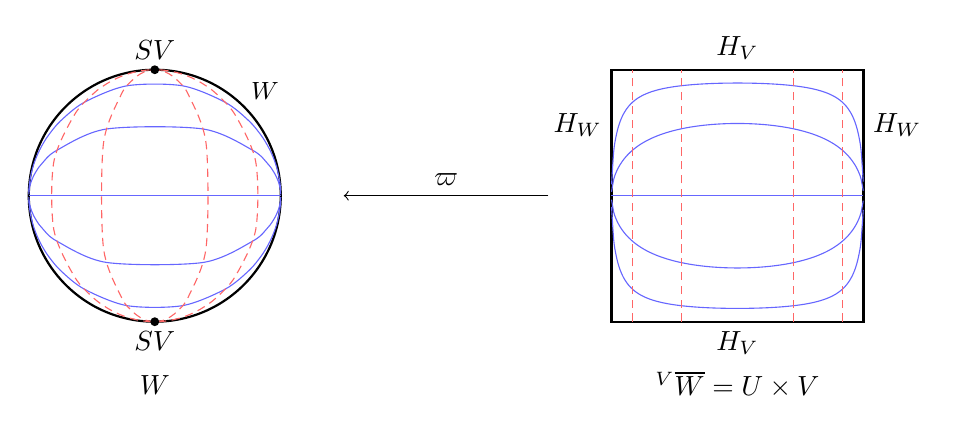
\begin{tikzpicture}[scale=1]
\begin{scope}
 \draw[thick] (0,0) circle (1.6);
 \foreach \c in {-2,-0.7,0.7,2}{
   \draw[blue!60,smooth,domain=-60:60,samples=120,variable=\t]
     plot ({1.6*\t/sqrt(1+\t*\t+\c*\c)},{1.6*\c/sqrt(1+\t*\t+\c*\c)});}
 \draw[blue!60] (-1.6,0)--(1.6,0);
 \foreach \c in {-1.5,-0.5,0.5,1.5}{
   \draw[red!60,densely dashed,smooth,domain=-60:60,samples=120,variable=\t]
     plot ({1.6*\c/sqrt(1+\t*\t+\c*\c)},{1.6*\t/sqrt(1+\t*\t+\c*\c)});}
 \fill (0,1.6) circle (1.6pt) node[above]{$SV$};
 \fill (0,-1.6) circle (1.6pt) node[below]{$SV$};
 \node at (0,-2.4) {$\RC W$};
 \node[above right] at (1.1,1.1) {\small$\pa\RC W$};
\end{scope}
\draw[->] (5.0,0)--(2.4,0) node[midway,above]{$\varpi$};
\begin{scope}[shift={(7.4,0)}]
 \draw[thick] (-1.6,-1.6) rectangle (1.6,1.6);
 \foreach \c in {-2,-0.7,0.7,2}{
   \draw[blue!60,smooth,domain=-0.999:0.999,samples=120,variable=\x]
     plot ({1.6*\x},{1.6*\c*sqrt(1-\x*\x)/sqrt(1+\c*\c*(1-\x*\x))});}
 \draw[blue!60] (-1.6,0)--(1.6,0);
 \foreach \c in {-1.5,-0.5,0.5,1.5}{
   \draw[red!60,densely dashed] ({1.6*\c/sqrt(1+\c*\c)},-1.6)--({1.6*\c/sqrt(1+\c*\c)},1.6);}
 \node[left] at (-1.6,0.9) {$H_W$};
 \node[right] at (1.6,0.9) {$H_W$};
 \node[above] at (0,1.6) {$H_V$};
 \node[below] at (0,-1.6) {$H_V$};
 \node at (0,-2.4) {$\RelC VW=\RC U\times\RC V$};
\end{scope}
\end{tikzpicture}
\caption{The relative compactification for $U=\R_\zeta$ (horizontal) and
$V=\R_\eta$ (vertical). The lines $\eta=\text{const}$ (solid) all end at the two
points $\zeta=\pm\infty$, $\eta/\ang\zeta=0$ of $H_W$; the lines
$\zeta=\text{const}$ (dashed), which in $\RC W$ all end at the two points of $SV$,
end at distinct points of the front faces $H_V$. The blow-down map $\varpi$
collapses each component of $H_V$ to a point of $SV$.}
\label{product:fig:relative}
\end{figure}

\begin{proposition}[Invariance]\label{product:prop:relative-invariance}
Let $\GL(W,V)=\{L\in\GL(W);L(V)=V\}$. The action of $\GL(W,V)$ on $W$ and the
action of $W$ on itself by translations extend to smooth actions
\begin{equation*}
\GL(W,V)\times\RelC VW\longrightarrow\RelC VW,\qquad W\times\RelC VW
\longrightarrow\RelC VW
\end{equation*}
by diffeomorphisms preserving $H_W$ and $H_V$. Consequently $\RelC VW$, with the
embedding $\iota_V$, is independent of the choice of $U$ and of the norms: two
choices give compactifications related by a unique diffeomorphism extending the
identity of $W$.
\end{proposition}

\begin{proof}
In terms of $W=U\oplus V$ an element $L\in\GL(W,V)$ is block lower triangular,
$L(\zeta,\eta)=(A\zeta,C\zeta+D\eta)$ with $A\in\GL(U)$, $D\in\GL(V)$, $C\in\Hom(U,V)$.
In the coordinates $(\zeta,q)$ of the interior, $L$ becomes
\begin{equation}\label{product:eq:lift-L}
(\zeta,q)\longmapsto\Big(A\zeta,\ g(\zeta)\Big(Dq+C\frac\zeta{\ang\zeta}\Big)\Big),
\qquad g(\zeta)=\frac{\ang\zeta}{\ang{A\zeta}}.
\end{equation}
Here $\zeta\mapsto A\zeta$ extends to a diffeomorphism of $\RC U$ by
\cref{product:lem:affine}, and $g$ and $\zeta/\ang\zeta$ are smooth on $\RC U$ (they
are classical symbols of order $0$), with $g>0$. So for fixed $\zeta\in\RC U$ the
second component is an invertible affine map of $V$ whose coefficients are smooth
on $\RC U$, and \cref{product:lem:affine} with $P=\RC U$ shows that
\eqref{product:eq:lift-L} extends to a diffeomorphism of $\RC U\times\RC V$; the
same argument with $P=\GL(W,V)\times\RC U$ gives joint smoothness of the action.
For a translation by $(a,c)$ the lifted map is
$(\zeta,q)\mapsto(\zeta+a,\ \tilde g(\zeta)(q+c/\ang\zeta))$ with
$\tilde g=\ang\zeta/\ang{\zeta+a}$, and the same argument applies. Finally,
changing the complement $U$ and the norms amounts to composing $\iota_V$ with an
element of $\GL(W,V)$.
\end{proof}

From \eqref{product:eq:lift-L} one sees that the boundary faces have some natural
structure. As $|q|\to\infty$ the direction of the second component tends to the
direction of $Dq$, so on $H_V$ the lifted action is $(\zeta,\theta)\mapsto
(A\zeta,D\theta/|D\theta|)$; thus there is a natural product decomposition
\begin{equation}\label{product:eq:HV}
H_V=\overline{W/V}\times SV.
\end{equation}
On the other hand on $H_W$ the action is $(\omega,q)\mapsto(A\omega/|A\omega|,
|\omega|_A^{-1}(Dq+C\omega))$, with $|\omega|_A=|A\omega|$; it covers the action
of $\GL(W/V)$ on $S(W/V)$, but the off-diagonal part $C$ acts on the fibres by
translations. Thus $H_W$ is naturally a fibration
\begin{equation}\label{product:eq:HW}
\RC V\text{---}H_W\longrightarrow S(W/V),
\end{equation}
trivial but not naturally a product, whose fibres are radial compactifications
of affine spaces modelled on $V$. In terms of the blow-up, $H_W=[SW;SV]$ and the
fibration is the extension $\gamma$ of $[w]\mapsto[w+V]$ (\cref{blowup:lem:sphere-fibration}).

\begin{proposition}\label{product:prop:blow-down}
\begin{enumerate}[label=\textup{(\roman*)}]
\item The identity of $W$ extends to a smooth surjective map
$\varpi:\RelC VW\longrightarrow\RC W$, the \emph{blow-down map}, with
$\varpi^*\rho=\rho_W\rho_V$ for $\rho=\ang{\zeta,\eta}^{-1}$. It restricts to a
diffeomorphism of $H_W\setminus H_V$ onto $SW\setminus SV$ and maps $H_V$ onto
$SV=\pa\RC V\subset\pa\RC W$, by the projection $\overline{W/V}\times SV
\longrightarrow SV$.
\item The projection $W\longrightarrow W/V$ extends to the fibration
$\RelC VW\longrightarrow\overline{W/V}$, with fibre $\RC V$, given in the product
description by projection onto the first factor; the inclusion $V\hookrightarrow
W$ extends to the embedding $\RC V\ni\eta\longmapsto(0,\eta)$ as the fibre over
$0$.
\end{enumerate}
\end{proposition}

\begin{proof}
In the half-sphere description of $\RC W$,
\begin{equation*}
\varpi(\zeta,q)=\Big(\frac1{\ang{\zeta,\eta}},\frac{\zeta}{\ang{\zeta,\eta}},
\frac{\eta}{\ang{\zeta,\eta}}\Big)=\Big(\rho_W\rho_V,\ \rho_V\frac\zeta{\ang\zeta},
\ \frac q{\ang q}\Big),
\end{equation*}
which is smooth on $\RC U\times\RC V$. On $H_V$ ($\rho_V=0$) the image is
$(0,0,\theta)$, $\theta=\lim q/|q|\in SV$. On $H_W\setminus H_V$ ($\rho_W=0$,
$\rho_V>0$) the image is $(0,\rho_V\omega,q/\ang q)$ with $\omega=\zeta/|\zeta|$,
$\rho_V=\ang q^{-1}$, a point of $SW$ with non-zero component in $U$; conversely
a point $(\hat\zeta,\hat\eta)\in SW$ with $\hat\zeta\ne0$ is the image of
$\omega=\hat\zeta/|\hat\zeta|$, $q=\hat\eta/|\hat\zeta|$, and this inverse is smooth.
Part (ii) is immediate from the definition.
\end{proof}

In fact $\varpi$ identifies $\RelC VW$ with the manifold obtained from $\RC W$ by
introducing polar coordinates around the submanifold $SV$ of its boundary, the
\emph{blow-up} $[\RC W;SV]$ (\cref{product:ex:blow-up}, proved in
\cref{blowup:thm:relative}): $SV$ is a p-submanifold of $\RC W$ of codimension
$k+1$, $H_V$ is the front face produced by the blow-up, and $H_W$ is the lift of the
original boundary, $H_W=[SW;SV]$.

\begin{remark}\label{product:rem:relative-bundle}
By \cref{product:prop:relative-invariance} the construction applies fibrewise to a
real vector bundle $W\longrightarrow X$ with a subbundle $V$: the transition maps
of local trivializations in which $V$ is trivialized as a subbundle take values in
$\GL(W,V)$, so the fibrewise relative compactifications form a compact (if $X$ is
compact) manifold with corners $\RelC VW$, fibred over $X$, with boundary faces
$H_W$ and $H_V$ and defining functions $\rho_W$, $\rho_V$ well defined up to
smooth positive factors. Moreover $H_V=\overline{W/V}\times_XSV$, and $H_W$
fibres over $S(W/V)$.
\end{remark}

\section{Product-type symbols}\label{product:sec:symbols}

We keep the notation $W=U\oplus V$, $w=(\zeta,\eta)$, $q=\eta/\ang\zeta$ of the
previous section, and let $\Omega\subset\R^p$ be an open set of parameters.
Estimates are required to hold uniformly for $x$ in compact subsets of $\Omega$.
For $M,M'\in\R$ define the weight
\begin{equation*}
w_{M,M'}(\zeta,\eta)=\ang q^{M}\ang\zeta^{M'}=\ang{\zeta,\eta}^{M}\ang\zeta^{M'-M}
=\rho_V^{-M}\rho_W^{-M'}.
\end{equation*}
The first order $M$ is the order at the front face $H_V$ and the second, $M'$,
the order at the main face $H_W$.

\begin{definition}\label{product:def:symbols}
The space $S^{M,M'}(\Omega;W,V)$ of \emph{product-type symbols} consists of the
$a\in\CI(\Omega\times W)$ such that for all multi-indices
\begin{equation}\label{product:eq:symbol-est}
|\pa_x^\gamma\pa_\zeta^\alpha\pa_\eta^\beta a(x,\zeta,\eta)|\le
C\ang\zeta^{M'-M-|\alpha|}\ang{\zeta,\eta}^{M-|\beta|}
=C\,w_{M,M'}(\zeta,\eta)\ang\zeta^{-|\alpha|}\ang{\zeta,\eta}^{-|\beta|}.
\end{equation}
The subspace of \emph{classical} (polyhomogeneous) product-type symbols is
\begin{equation*}
S^{M,M'}_{\mathrm{ph}}(\Omega;W,V)=\{a;\ a=\rho_V^{-M}\rho_W^{-M'}b\ \text{on }
\Omega\times W,\ b\in\CI(\Omega\times\RelC VW)\}.
\end{equation*}
\end{definition}

By \cref{product:prop:relative-invariance}, $S^{M,M'}_{\mathrm{ph}}$ does not depend
on the choices made, since the defining functions change by smooth positive
factors; we shall see in \cref{product:prop:symbols}(vii) that the same is true of
$S^{M,M'}$. Thus $\ang{\zeta,\eta}^\mu\in S^{\mu,\mu}_{\mathrm{ph}}$, while
$\ang\zeta^\mu\in S^{0,\mu}_{\mathrm{ph}}$ is constant along $V$. Each
$\pa_\zeta$-derivative improves the estimate by $\ang\zeta^{-1}$, each
$\pa_\eta$-derivative by $\ang{\zeta,\eta}^{-1}$.

\begin{discussion}
  The two orders measure growth in two different regimes. Near the main face
  $H_W$, $|\zeta|$ is large and $\eta$ is at most comparable to $\zeta$: this is
  where an ordinary symbol of order $M'$ lives. Near the front face $H_V$, $\eta$
  is much larger than $\zeta$: the symbol grows like $|\eta|^M$ and, for fixed
  direction of $\eta$, is a symbol of order $M'-M$ in $\zeta$. The estimate
  \eqref{product:eq:symbol-est} is the standard symbol estimate with these two
  regimes separated: $\pa_\zeta$ gains only $\ang\zeta^{-1}$, not
  $\ang{\zeta,\eta}^{-1}$.
\end{discussion}

\begin{lemma}[Peetre's inequality]\label{product:lem:peetre}
For all $M,M'$ there is $C$ such that for all $w,\theta\in W$
\begin{equation*}
w_{M,M'}(w+\theta)\le C\,w_{M,M'}(w)\ang\theta^{|M|+|M'-M|}.
\end{equation*}
\end{lemma}

\begin{proof}
Apply Peetre's inequality $\ang{x+y}^s\le2^{|s|/2}\ang x^s\ang y^{|s|}$ to each
factor of $\ang{\zeta,\eta}^M\ang\zeta^{M'-M}$.
\end{proof}

\begin{proposition}\label{product:prop:symbols}
\begin{enumerate}[label=\textup{(\roman*)}]
\item $a\in S^{M,M'}(\Omega;W,V)$ if and only if $c(x,\zeta,q)=a(x,\zeta,\ang\zeta q)$
satisfies the product estimates
\begin{equation*}
|\pa_x^\gamma\pa_\zeta^\alpha\pa_q^\beta c|\le C\ang\zeta^{M'-|\alpha|}\ang
q^{M-|\beta|}.
\end{equation*}
\item $S^{M,M'}_{\mathrm{ph}}\subset S^{M,M'}$.
\item $S^{M_1,M_1'}\cdot S^{M_2,M_2'}\subset S^{M_1+M_2,M_1'+M_2'}$, and the same
for classical symbols.
\item $\pa_\zeta:S^{M,M'}\longrightarrow S^{M,M'-1}$ and
$\pa_\eta:S^{M,M'}\longrightarrow S^{M-1,M'-1}$, and the same for classical
symbols. Moreover $S^{M,M'}\subset S^{M+1,M'}\cap S^{M,M'+1}$ and
$S^{M-1,M'-1}\subset S^{M,M'-1}$, and the same inclusions hold for classical
symbols. More generally $S^{M,M'}\subset S^{M+s,M'+s'}$ for all real $s,s'\ge0$,
but $S^{M,M'}_{\mathrm{ph}}\subset S^{M+s,M'+s'}_{\mathrm{ph}}$ only for
$s,s'\in\N_0$: for instance $1\in S^{0,0}_{\mathrm{ph}}$ is not in
$S^{1/2,0}_{\mathrm{ph}}$, since $\rho_V^{1/2}$ is not smooth.
\item The standard symbols on $W$ are included: $\Sym\mu(\Omega;W)\subset
S^{\mu,\mu}(\Omega;W,V)$ and $\Symph\mu(\Omega;W)\subset
S^{\mu,\mu}_{\mathrm{ph}}(\Omega;W,V)$; more precisely
$\Symph\mu(\Omega;W)=\varpi^*\big(\rho^{-\mu}\CI(\Omega\times\RC W)\big)$.
\item Symbols on $W/V$ lift: if $a\in\Sym\mu(\Omega;W/V)$ then
$a(x,\zeta)\in S^{0,\mu}(\Omega;W,V)$, and similarly for classical symbols.
\item If $L\in\CI(\Omega;\GL(W,V))$ and $a\in S^{M,M'}$ then $a(x,L(x)w)\in
S^{M,M'}$, and the same for classical symbols.
\item The residual spaces are
\begin{gather*}
S^{M,-\infty}=\bigcap_{M'}S^{M,M'}=\cS(U;\Sym M(\Omega;V)),\quad
S^{M,-\infty}_{\mathrm{ph}}=\bigcap_{M'}S^{M,M'}_{\mathrm{ph}}=
\cS(U;\Symph M(\Omega;V)),\\
S^{-\infty,-\infty}=\bigcap_{M,M'}S^{M,M'}=\bigcap_{M,M'}S^{M,M'}_{\mathrm{ph}}
=\CI(\Omega;\cS(W)),
\end{gather*}
where $\cS(U;\Sym M(\Omega;V))$ consists of the $a$ with $|\pa_x^\gamma
\pa_\zeta^\alpha\pa_\eta^\beta a|\le C_N\ang\zeta^{-N}\ang\eta^{M-|\beta|}$ for all
$N$, and the classical version requires in addition that
$a(x,\zeta,\cdot)$ be classical, with all terms of the expansion rapidly
decreasing in $\zeta$.
\end{enumerate}
\end{proposition}

\begin{proof}
(i) Consider the vector fields $L_j=\ang\zeta\pa_{\zeta_j}$ and
$Q_i=\ang{\zeta,\eta}\pa_{\eta_i}$ in the coordinates $(\zeta,\eta)$, and
$L'_j=\ang\zeta\pa_{\zeta_j}$, $Q'_i=\ang q\pa_{q_i}$ in the coordinates
$(\zeta,q)$. Since $\pa_q=\ang\zeta\pa_\eta$ and $\ang q\ang\zeta=\ang{\zeta,\eta}$,
\begin{equation*}
Q'_i=Q_i,\qquad L'_j=L_j+\frac{\zeta_j}{\ang\zeta}\sum_i\frac{q_i}{\ang q}Q_i.
\end{equation*}
The functions $\zeta_j/\ang\zeta$ and $q_i/\ang q$ are annihilated by $Q'$,
respectively $L'$, and any number of applications of $L'$, respectively $Q'$, to
them gives bounded functions of the same type. Hence the products of $L$'s and
$Q$'s, and the products of $L'$'s and $Q'$'s, are linear combinations of each
other with bounded coefficients all of whose $L'$, $Q'$ derivatives are bounded.
By the usual induction, the estimates \eqref{product:eq:symbol-est} are equivalent
to $|P a|\le Cw_{M,M'}$ for all products $P$ of the $L_j$, $Q_i$ and $\pa_x$
(using $\pa^\alpha_\zeta=\ang\zeta^{-|\alpha|}L^\alpha+$ lower order terms with
coefficients which are bounded symbols of negative order, and similarly for
$\eta$), and the product estimates are equivalent to $|P'c|\le Cw_{M,M'}$ for all
products $P'$ of the $L'_j$, $Q'_i$ and $\pa_x$. This proves (i).

(ii) If $b\in\CI(\Omega\times\RC U\times\RC V)$ then $L'_j$ and $Q'_i$ lift to
smooth vector fields on $\RC U\times\RC V$ (they are tangent to the boundary), so
$P'b$ is bounded for every product $P'$. The weight $\ang\zeta^{M'}\ang q^{M}$ is
itself a product-type symbol in the sense of (i), so (ii) follows from (i) and
Leibniz' formula.

(iii) and (iv) follow directly from \eqref{product:eq:symbol-est} and Leibniz'
formula, and for classical symbols from the fact that $L'_j$, $Q'_i$, and hence
$\rho_W^{-1}\pa_{\zeta_j}=L_j$ and $(\rho_W\rho_V)^{-1}\pa_{\eta_i}=Q_i$ (in the
original coordinates), are smooth vector fields on $\RelC VW$ tangent to the
boundary; the inclusions in (iv) hold because $\ang q\ge1$ and $\ang\zeta\ge1$,
and in the classical case because $\rho_V^{-M}\rho_W^{-M'}b=
\rho_V^{-M-j}\rho_W^{-M'-k}(\rho_V^j\rho_W^kb)$ for $j,k\in\N_0$. If
$1=\rho_V^{-1/2}b$ with $b$ smooth then $b=\rho_V^{1/2}$ near the interior of
$H_V$, which is not smooth.

(v) For $a\in\Sym\mu(W)$, $|\pa^\alpha_\zeta\pa^\beta_\eta a|\le
C\ang{\zeta,\eta}^{\mu-|\alpha|-|\beta|}\le C\ang\zeta^{-|\alpha|}
\ang{\zeta,\eta}^{\mu-|\beta|}$, which is \eqref{product:eq:symbol-est} with
$M=M'=\mu$. The classical statement follows from \cref{product:prop:blow-down}(i)
since $\varpi^*\rho=\rho_V\rho_W$.

(vi) is clear from (i), since $c$ is independent of $q$; for classical symbols
use \cref{product:prop:blow-down}(ii).

(vii) If $L(x)(\zeta,\eta)=(A\zeta,C\zeta+D\eta)$ then by the chain rule
$\pa_\eta(a\circ L)=D^t(\pa_\eta a)\circ L$ and $\pa_\zeta(a\circ L)=
A^t(\pa_\zeta a)\circ L+C^t(\pa_\eta a)\circ L$, and $x$-derivatives produce
similar terms with coefficients $\pa_xA$, etc. Using (iv) and the fact that
$w_{M,M'}\circ L$ is bounded above and below by multiples of $w_{M,M'}$ (since
$\ang{A\zeta}\simeq\ang\zeta$ and $\ang{L(\zeta,\eta)}\simeq\ang{\zeta,\eta}$, locally
uniformly in $x$), the estimates follow by induction. The classical case follows
from the smoothness of the action in \cref{product:prop:relative-invariance}.

(viii) Since $\ang\zeta^{-N-M}\ang{\zeta,\eta}^{M-|\beta|}$ lies between
$\ang\zeta^{-N-M\mp|M-|\beta||}\ang\eta^{M-|\beta|}$ (by Peetre's inequality in the
form $\ang\eta^s\ang\zeta^{-|s|}\le\ang{\zeta,\eta}^s\le\ang\eta^s\ang\zeta^{|s|}$),
the first identity is clear. For the classical case, $a\in
S^{M,M'}_{\mathrm{ph}}$ for all $M'$ means that $a=\ang q^Mb(\zeta,q)$ where $b$ is
smooth on $\RC U\times\RC V$ and vanishes to infinite order at
$H_W=SU\times\RC V$, i.e.\ $b$ is a Schwartz function of $\zeta$ with values in
the Fréchet space $\CI(\RC V)$. For fixed $\zeta$, $\eta\mapsto a(\zeta,\eta)$ is
obtained from $\ang q^Mb(\zeta,q)\in\rho_V^{-M}\CI(\RC V)=\Symph M(V)$ by the
dilation $q=\eta/\ang\zeta$. Dilations by $\lambda\in(0,1]$ act on $\Symph M(V)$
with each seminorm bounded by $C\lambda^{-K}$ times a seminorm, so
$a\in\cS(U;\Symph M(V))$; the converse is proved in the same way using the
inverse dilation. Finally, taking $M=M'=-N$ gives $w_{M,M'}=\ang{\zeta,\eta}^{-N}$,
so $S^{-\infty,-\infty}$ consists of Schwartz functions; conversely
$w_{M,M'}\ge\ang{\zeta,\eta}^{-|M|-|M'-M|}$, so Schwartz functions lie in every
$S^{M,M'}$, and they are classical, being $\rho^\infty\CI(\RC W)$ lifted by $\varpi$.
\end{proof}

\begin{lemma}[Translations]\label{product:lem:translation}
For $\theta\in W$ the translation $a\longmapsto a(\cdot+\theta)$ maps
$S^{M,M'}_{\mathrm{ph}}(\Omega;W,V)$ and $S^{M,M'}(\Omega;W,V)$ into themselves;
each seminorm of $a(\cdot+\theta)$ is bounded by $C\ang\theta^K$ times a seminorm
of $a$.
\end{lemma}

\begin{proof}
For $S^{M,M'}$ this is \cref{product:lem:peetre} applied to
\eqref{product:eq:symbol-est}. For classical symbols, the translation lifts to a
diffeomorphism $T_\theta$ of $\RelC VW$ depending smoothly on $\theta$
(\cref{product:prop:relative-invariance}) and preserving the boundary faces, so
$T_\theta^*(\rho_V^{-M}\rho_W^{-M'})/(\rho_V^{-M}\rho_W^{-M'})$ is smooth and
positive. From the explicit form $(\zeta,q)\mapsto(\zeta+\theta_1,
\ang\zeta\ang{\zeta+\theta_1}^{-1}(q+\theta_2/\ang\zeta))$ one checks, using the
coordinates of \cref{product:prop:relative-coords}, that all derivatives of
$T_\theta$ and of this quotient are bounded by powers of $\ang\theta$.
\end{proof}

\begin{proposition}[Asymptotic completeness]\label{product:prop:asymptotic}
\begin{enumerate}[label=\textup{(\roman*)}]
\item If $a_j\in S^{M,M'-j}_{\mathrm{ph}}(\Omega;W,V)$ for $j\in\N_0$, there is
$a\in S^{M,M'}_{\mathrm{ph}}$ with $a-\sum_{j<N}a_j\in S^{M,M'-N}_{\mathrm{ph}}$ for
all $N$; $a$ is unique modulo $S^{M,-\infty}_{\mathrm{ph}}$.
\item If $a_j\in S^{M-j,M'}_{\mathrm{ph}}$, there is $a\in S^{M,M'}_{\mathrm{ph}}$ with
$a-\sum_{j<N}a_j\in S^{M-N,M'}_{\mathrm{ph}}$ for all $N$; $a$ is unique modulo
$S^{-\infty,M'}_{\mathrm{ph}}=\bigcap_jS^{M-j,M'}_{\mathrm{ph}}$.
\item If $a_j\in S^{M-j,M'-j}_{\mathrm{ph}}$, there is $a\in S^{M,M'}_{\mathrm{ph}}$
with $a-\sum_{j<N}a_j\in S^{M-N,M'-N}_{\mathrm{ph}}$ for all $N$; $a$ is unique
modulo $S^{-\infty,-\infty}$.
\end{enumerate}
The same statements hold for the spaces $S^{M,M'}$.
\end{proposition}

\begin{proof}
Write $a_j=\rho_V^{-M}\rho_W^{-M'}\rho_W^jb_j$ in case (i). Near $H_W$ the factor
$\RC U$ has a collar $[0,1)_{\rho_W}\times SU$, so $\RelC VW$ has a collar
$[0,1)\times H_W$, and Borel's lemma (with parameters in $\Omega\times H_W$) gives
$b\in\CI(\Omega\times\RelC VW)$ with $b-\sum_{j<N}\rho_W^jb_j\in\rho_W^N\CI$ for
all $N$: take $b=\sum_j\chi(\rho_W/\eps_j)\rho_W^jb_j$ with $\chi\in\CIc([0,1))$
equal to $1$ near $0$ and $\eps_j\downarrow0$ so fast that the $j$-th term has
$C^{j-1}$ norm at most $2^{-j}$ on $K_j\times\RelC VW$, where $K_1\subset
K_2\subset\cdots$ is an exhaustion of $\Omega$ by compact sets. This is possible:
since $|\pa^\alpha(\chi(\rho_W/\eps))|\le C_\alpha\eps^{-|\alpha|}$ and
$\rho_W\le\eps$ on the support, each derivative of order $k$ of
$\chi(\rho_W/\eps)\rho_W^jb_j$ is $O(\eps^{j-k})$, which is small for $k\le j-1$.
(One cannot ask for smallness in $C^j$: $\pa_{\rho_W}^j(\chi(\rho_W/\eps)\rho_W^jb_j)
=j!\,b_j$ at $\rho_W=0$, whatever $\eps$.) For each $k$ the terms with $j>k$ are
then summable in $C^k$ on each $K_i\times\RelC VW$, so the series converges in
$\CI$. Given $N$,
\begin{equation*}
b-\sum_{j<N}\rho_W^jb_j=\sum_{j<N}(\chi(\rho_W/\eps_j)-1)\rho_W^jb_j
+\sum_{j\ge N}\chi(\rho_W/\eps_j)\rho_W^jb_j.
\end{equation*}
The first sum vanishes near $H_W$. Each term of the second vanishes to order $N$
at $H_W$, i.e.\ its derivatives of order $<N$ in the collar variable $\rho_W$
vanish at $\rho_W=0$; by convergence in $\CI$ the same holds for the sum, which
is therefore $\rho_W^N$ times a smooth function by Taylor's formula with integral
remainder in the collar. Then $a=\rho_V^{-M}\rho_W^{-M'}b$. Uniqueness holds since
the difference of two choices vanishes to infinite order at $H_W$. Case (ii) is
the same with $\rho_V$ in place of $\rho_W$, and case (iii) the same with
$\rho=\rho_V\rho_W$ in the cut-offs: the $C^k$ norm of $\rho^j\chi(\rho/\eps)b_j$
is again $O(\eps^{j-k})$, and the tail $g=\sum_{j\ge N}\chi(\rho/\eps_j)\rho^jb_j$
vanishes to order $N$ at both faces. By the one-face argument $g=\rho_W^Ng_1$ with
$g_1$ smooth; $g_1=\rho_W^{-N}g$ vanishes to order $N$ at $H_V\setminus H_W$, where
$\rho_W>0$, hence by continuity of its derivatives at all of $H_V$, so
$g_1=\rho_V^Ng_2$ and $g\in\rho^N\CI$. For non-classical symbols one uses instead the usual
cut-offs $1-\chi(\ang\zeta/R_j)$, $1-\chi(\ang q/R_j)$, respectively
$1-\chi(\ang{\zeta,\eta}/R_j)$, with $R_j\to\infty$ rapidly, exactly as for
standard symbols.
\end{proof}

\subsection{Symbol maps in the model case}
For $a\in S^{M,M'}_{\mathrm{ph}}(\Omega;W,V)$, $a=\rho_V^{-M}\rho_W^{-M'}b$, the
restrictions of $b$ to the two boundary faces are given by limits. For $w=(\zeta,\eta)$
with $\zeta\ne0$ (that is, $w\notin V$) and for $\eta\in V\setminus0$, put
\begin{equation}\label{product:eq:model-symbols}
\sigma_W(a)(x,w)=\lim_{t\to\infty}t^{-M'}a(x,tw),\qquad
\sigma_V(a)(x,\zeta,\eta)=\lim_{t\to\infty}t^{-M}a(x,\zeta,t\eta).
\end{equation}
Using $\ang{tw}\simeq t|w|$ and $tq\to\infty$ one finds
\begin{equation*}
\sigma_W(a)(x,w)=|\zeta|^{M'-M}|w|^Mb\big(x,\tfrac\zeta{|\zeta|},\tfrac\eta{|\zeta|}\big),\qquad
\sigma_V(a)(x,\zeta,\eta)=\ang\zeta^{M'-M}|\eta|^Mb\big(x,\zeta,\tfrac\eta{|\eta|}\big),
\end{equation*}
where $(\zeta/|\zeta|,\eta/|\zeta|)\in SU\times V$ is a point of the interior of
$H_W$ and $(\zeta,\eta/|\eta|)$ a point of $H_V=\RC U\times SV$, and $|w|$ is the
Euclidean norm on $W=U\oplus V$. Thus $\sigma_W(a)$ is homogeneous of degree $M'$
on $W\setminus V$, while for each $\eta\ne0$, $\sigma_V(a)(x,\cdot,\eta)$ is a
classical symbol of order $M'-M$ on $U=W/V$, and $\sigma_V(a)$ is homogeneous of
degree $M$ in $\eta$. Let $\Sigma_W^{M,M'}$ and $\Sigma_V^{M,M'}$ denote the
spaces of such functions, i.e.\ of the functions $s$ of this form with $b$ a
smooth function on $\Omega\times H_W$, respectively $\Omega\times H_V$.

\begin{lemma}\label{product:lem:model-symbol-maps}
The maps $\sigma_W$ and $\sigma_V$ give short exact sequences
\begin{gather*}
S^{M,M'-1}_{\mathrm{ph}}\hookrightarrow S^{M,M'}_{\mathrm{ph}}\overset{\sigma_W}
\longrightarrow\Sigma_W^{M,M'},\qquad
S^{M-1,M'}_{\mathrm{ph}}\hookrightarrow S^{M,M'}_{\mathrm{ph}}\overset{\sigma_V}
\longrightarrow\Sigma_V^{M,M'},\\
S^{M-1,M'-1}_{\mathrm{ph}}\hookrightarrow S^{M,M'}_{\mathrm{ph}}
\xrightarrow{(\sigma_W,\sigma_V)}\{(s_W,s_V)\in\Sigma_W^{M,M'}\times\Sigma_V^{M,M'};
\ \text{\eqref{product:eq:compatibility} holds}\},
\end{gather*}
where the compatibility condition, which expresses the equality of the restrictions
of $b|_{H_W}$ and $b|_{H_V}$ to the corner, is
\begin{equation}\label{product:eq:compatibility}
\lim_{t\to\infty}t^{-M}s_W(x,\zeta+t\eta)=\lim_{r\to\infty}r^{M-M'}s_V(x,r\zeta,\eta),
\qquad\zeta\in U\setminus0,\ \eta\in V\setminus0;
\end{equation}
that is, the leading homogeneous term of $s_W$ at $V$ is the principal symbol of
the classical symbol $s_V(x,\cdot,\eta)$ on $U$.
\end{lemma}

\begin{proof}
$b|_{H_W}=0$ if and only if $b\in\rho_W\CI$, which gives the null space of
$\sigma_W$, and similarly for $\sigma_V$. If $b$ vanishes on both faces then
$b=\rho_Vb'$ with $b'$ vanishing on $H_W\setminus H_V$, hence by continuity on
$H_W$, so $b=\rho_V\rho_Wb''$. For surjectivity use the product structure: if
$c_V\in\CI(\Omega\times\RC U\times SV)$ and $c_W\in\CI(\Omega\times SU\times\RC V)$
agree on $SU\times SV$, let $\chi\in\CIc([0,1))$ be $1$ near $0$, set
$\tilde c_V(x,\zeta,q)=\chi(\rho_V)c_V(x,\zeta,q/|q|)$ and
\begin{equation*}
b=\tilde c_V+\chi(\rho_W)\big(c_W-\tilde c_V|_{H_W}\big)(x,\zeta/|\zeta|,q).
\end{equation*}
Then $b|_{H_V}=c_V$, since $c_W-\tilde c_V|_{H_W}$ vanishes at the corner, and
$b|_{H_W}=c_W$. This construction needs the compatibility: if, say, $c_V$ is
non-zero at the corner then no $b$ has $b|_{H_V}=c_V$ and $b|_{H_W}=0$. For the
separate maps no compatibility is needed: given $c_V$ alone, $\tilde c_V$ restricts
to $c_V$ on $H_V$ (its restriction to $H_W$ being whatever it is), and given $c_W$
alone, $\chi(\rho_W)c_W(x,\zeta/|\zeta|,q)$ restricts to $c_W$ on $H_W$. So the
separate maps are surjective. The computation of the limits above shows
that the compatibility of $b|_{H_W}$ and $b|_{H_V}$ at the corner is
\eqref{product:eq:compatibility}.
\end{proof}

\section{Product-type conormal distributions}\label{product:sec:conormal}

Let $Z\subset Y\subset X$ be closed embedded submanifolds of a manifold $X$ of
dimension $n$, with $\dim Z=d$, $\dim Y=d+k$, so that $Z$ has codimension $k$ in $Y$
and $Y$ has codimension $l=n-d-k$ in $X$. (In this section $Z$ denotes a
submanifold, not the fibre of a fibration.) We define spaces
$\Ic{m,m'}(X,Y,Z;E)$ of distributions which are conormal to $Y$ of order $m$ and,
in a product sense, conormal to $Z$ of order $m'$. Thus the \emph{first} index
refers to the larger submanifold $Y$.

\begin{figure}[ht]
\centering
\begin{tikzpicture}[>=Stealth]
\fill[gray!15] (-2.6,-0.6)--(2.2,-0.6)--(3.4,0.6)--(-1.4,0.6)--cycle;
\draw (-2.6,-0.6)--(2.2,-0.6)--(3.4,0.6)--(-1.4,0.6)--cycle;
\draw[line width=1.8pt] (-2.0,0)--(2.8,0);
\draw[->] (-1.4,-1.6)--(-1.4,1.6) node[above,font=\footnotesize]{$y$ (normal to $Y$)};
\draw[->] (-0.8,-0.3)--(0.0,0.5);
\node[font=\footnotesize] at (0.3,0.75) {$z$ (in $Y$, normal to $Z$)};
\draw[->] (0.6,-0.35)--(1.4,-0.35) node[right,font=\footnotesize]{$w$};
\node[font=\small,above right] at (2.8,0) {$Z$};
\node[font=\small] at (-1.95,-0.38) {$Y$};
\node[font=\small] at (3.3,1.4) {$X$};
\node[font=\footnotesize,align=left,anchor=west] at (4.2,0.6)
  {away from $Z$: conormal to $Y$,\\ symbol in $\eta$ of order $M$};
\node[font=\footnotesize,align=left,anchor=west] at (4.2,-0.5)
  {at $Z$: product-type symbol\\ in $(\zeta,\eta)$ of orders $(M,M')$};
\end{tikzpicture}
\caption{The nested pair $Z\subset Y\subset X$ in adapted coordinates
$(w,z,y)$: $Y=\{y=0\}$ (shaded) and $Z=\{z=y=0\}$ (thick line). The dual
variables are $\zeta$ (to $z$) and $\eta$ (to $y$). A product-type conormal
distribution is conormal to $Y$ away from $Z$ (for instance a $\delta$-function in
the directions normal to $Y$) and has an additional conormal singularity along $Z$.
For the fibrewise and product-type operators, $X=M^2$, $Y=M^2_\phi$ and
$Z=\Diag_M$.}
\label{product:fig:nested}
\end{figure}

\subsection{The model case}
Let $X=\R^n=\R^d_w\times\R^k_z\times\R^l_y$, $Y=\{y=0\}$, $Z=\{z=0,y=0\}$. The
conormal space to $Z$ at each point is $W=\R^k_\zeta\times\R^l_\eta$, the dual
of the normal variables $(z,y)$, and the conormal space to $Y$ is its subspace
$V=\{\zeta=0\}$, the annihilator of the $z$-directions; the quotient $W/V\cong
\R^k_\zeta$ is the conormal space of $Z$ in $Y$. For a compactly supported
distribution $u$ we write
$\hat u(w,\zeta,\eta)=\int e^{-i(z\cdot\zeta+y\cdot\eta)}u(w,z,y)\,dz\,dy$ for the
partial Fourier transform in the normal variables. Set
\begin{equation}\label{product:eq:orders}
M=m+\frac n4-\frac l2,\qquad M'=m'+\frac n4-\frac{k+l}2;
\end{equation}
these are the symbol orders corresponding, with the normalization of
\cref{ch:conormal}, to conormal order $m$ at $Y$ and $m'$ at $Z$.

\emph{Convention.} Since product-type symbols are weighted smooth functions, the
spaces of conormal distributions which they contain are the classical ones.
\emph{In this section, $\Ic m(\Omega,Y)$, $\Ic{m'}(\Omega,Z)$, $\Ic m(X,Y;E)$, etc.\
denote the classical spaces $\Ic m_{\mathrm{ph}}$ of \cref{ch:conormal}}; the
corresponding statements for the general spaces are false (for instance a
non-classical element of $\Ic m(X,Y)$ is not in any $\Ic{m,m'}(X,Y,Z)$).

Recall from
\cref{ch:conormal} that, in these coordinates, $u\in\Ic m(\Omega,Y)$ if and only
if for each $\chi\in\CIc(\Omega)$ the partial Fourier transform of $\chi u$ in $y$
alone is a classical symbol of order $M$ in $\eta$, depending smoothly on $(w,z)$,
and $u\in\Ic{m'}(\Omega,Z)$ if and only if each $\widehat{\chi u}$ lies in
$\Symph{M'}(\R^d;W)$.

\begin{definition}\label{product:def:model-conormal}
For $\Omega\subset\R^n$ open, $\Ic{m,m'}(\Omega,Y,Z)$ is the space of
$u\in\CmI(\Omega)$ such that for every $\chi\in\CIc(\Omega)$,
$\widehat{\chi u}\in S^{M,M'}_{\mathrm{ph}}(\R^d;W,V)$, with $M,M'$ given by
\eqref{product:eq:orders}.
\end{definition}

Thus, for $\chi\in\CIc(\Omega)$, $\chi u=\int e^{i(z\cdot\zeta+y\cdot\eta)}
a(w,\zeta,\eta)\,\dbar\zeta\,\dbar\eta$ (an oscillatory integral) with
$a=\widehat{\chi u}$ a product-type symbol, compactly supported in $w$. The
definition is local: if $u\in\Ic{m,m'}(\Omega,Y,Z)$ and $\psi\in\CI(\Omega)$
then $\psi u\in\Ic{m,m'}(\Omega,Y,Z)$, and membership can be checked using
$\chi$'s from a partition of unity. The basic tool for handling these
distributions is the following reduction of amplitudes.

\begin{lemma}[Amplitudes]\label{product:lem:amplitude}
Let $r\in S^{M,M'}_{\mathrm{ph}}(\R^n;W,V)$ have support in $K\times W$ for a
compact $K\subset\R^n$, and let
\begin{equation*}
v(x)=\int e^{i(z\cdot\zeta+y\cdot\eta)}r(x,\zeta,\eta)\,\dbar\zeta\,\dbar\eta,
\quad x=(w,z,y),
\end{equation*}
as an oscillatory integral. Then $\hat v\in S^{M,M'}_{\mathrm{ph}}(\R^d;W,V)$ and,
with $\xi=(\zeta,\eta)$,
\begin{equation}\label{product:eq:amplitude-expansion}
\hat v(w,\xi)\sim\sum_{\gamma}\frac1{\gamma!}(-D_\xi)^\gamma\pa_{(z,y)}^\gamma
r(w,0,0,\xi),
\end{equation}
in the sense that the difference between $\hat v$ and the sum over
$|\gamma|<N$ is in $S^{M,M'-N}$ for every $N$. The terms with $\gamma=(\alpha,0)$
lie in $S^{M,M'-|\alpha|}_{\mathrm{ph}}$, those with $\gamma=(\alpha,\beta)$,
$\beta\ne0$, in $S^{M-1,M'-|\gamma|}_{\mathrm{ph}}$.
In particular $v\in\Ic{m,m'}(\R^n,Y,Z)$.
\end{lemma}

\begin{proof}
Let $\tilde r(w,\theta;\xi)=\int e^{-i(z,y)\cdot\theta}r(w,z,y,\xi)\,dz\,dy$ be the
Fourier transform of $r$ in $(z,y)$; since $r$ has compact support in $x$ and
satisfies the estimates \eqref{product:eq:symbol-est} with all $x$-derivatives,
integration by parts shows that for each $L$ the family
$\ang\theta^L\tilde r(\cdot,\theta;\cdot)$, $\theta\in\R^{k+l}$, is bounded in
$S^{M,M'}_{\mathrm{ph}}(\R^d;W,V)$; that is, $\tilde r$ is rapidly decreasing in
$\theta$ with values in $S^{M,M'}_{\mathrm{ph}}$. Inserting the definition of $v$ and integrating first in
$(z,y)$ (which is justified by inserting a cut-off $\chi(\eps\xi)$ and letting
$\eps\to0$),
\begin{equation*}
\hat v(w,\xi)=\int\tilde r(w,\xi-\xi';\xi')\,\dbar\xi'=\int\tilde r(w,\theta;\xi-\theta)
\,\dbar\theta.
\end{equation*}
By \cref{product:lem:translation} the integrand is, for each $\theta$, in
$S^{M,M'}_{\mathrm{ph}}$ with seminorms bounded by $C_L\ang\theta^{K-L}$, so the
integral converges in $S^{M,M'}_{\mathrm{ph}}$ and $\hat v$ is a classical
product-type symbol. For the expansion, apply Taylor's formula in the last
variable:
\begin{equation*}
\tilde r(w,\theta;\xi-\theta)=\sum_{|\gamma|<N}\frac{(-\theta)^\gamma}{\gamma!}
\pa_\xi^\gamma\tilde r(w,\theta;\xi)+\sum_{|\gamma|=N}\frac{N(-\theta)^\gamma}{\gamma!}
\int_0^1(1-s)^{N-1}\pa_\xi^\gamma\tilde r(w,\theta;\xi-s\theta)\,ds.
\end{equation*}
Since $\int\theta^\gamma\tilde r(w,\theta;\xi)\,\dbar\theta=D^\gamma_{(z,y)}r(w,0,0,\xi)$,
the terms with $|\gamma|<N$ give the sum in \eqref{product:eq:amplitude-expansion},
noting $(-\pa_\xi)^\gamma D^\gamma=(-D_\xi)^\gamma\pa^\gamma$. By
\cref{product:prop:symbols}(iv), $\pa_\xi^\gamma r\in S^{M,M'-N}$ when $|\gamma|=N$,
so by \cref{product:lem:peetre} the remainder is bounded by
$C\int\ang\theta^{-L}w_{M,M'-N}(\xi-s\theta)\,d\theta\le C'w_{M,M'-N}(\xi)$, and the
same argument applies to its derivatives. The orders of the individual terms
follow from \cref{product:prop:symbols}(iv), since $(-D_\xi)^\gamma$ contains at
least one $\eta$-derivative if $\beta\ne0$.
\end{proof}

\begin{proposition}\label{product:prop:model-properties}
Let $\Omega\subset\R^n$ be open.
\begin{enumerate}[label=\textup{(\roman*)}]
\item $\Ic m(\Omega,Y)\subset\Ic{m,-\infty}(\Omega,Y,Z)=\bigcap_{m'}
\Ic{m,m'}(\Omega,Y,Z)$, with equality, and
$\Ic{m'}(\Omega,Z)\subset\Ic{m'-k/2,m'}(\Omega,Y,Z)$.
\item $\bigcap_j\Ic{m-j,m'-j}(\Omega,Y,Z)=\CI(\Omega)$.
\item If $u\in\Ic{m,m'}(\Omega,Y,Z)$ then $u|_{\Omega\setminus Z}\in
\Ic m(\Omega\setminus Z,Y\setminus Z)$; in particular $u$ is smooth off $Y$.
\item Multiplication by $y_j$ maps $\Ic{m,m'}$ into $\Ic{m-1,m'-1}$, multiplication
by $z_j$ maps it into $\Ic{m,m'-1}$, and smooth vector fields tangent to both $Y$
and $Z$ map $\Ic{m,m'}$ into itself.
\end{enumerate}
\end{proposition}

\begin{proof}
(i) If $u\in\Ic m(\Omega,Y)$ and $\chi\in\CIc(\Omega)$, the partial Fourier
transform of $\chi u$ in $y$ is a classical symbol of order $M$ in $\eta$ which is
smooth and compactly supported in $(w,z)$; its Fourier transform in $z$ is
therefore in $\cS(\R^k_\zeta;\Symph M(\R^d;\R^l))=S^{M,-\infty}_{\mathrm{ph}}$ by
\cref{product:prop:symbols}(viii). Conversely, if $\widehat{\chi u}\in
S^{M,-\infty}_{\mathrm{ph}}$ then its inverse Fourier transform in $\zeta$ is
smooth in $(w,z)$ and a classical symbol in $\eta$, so $\chi u\in\Ic m(\Omega,Y)$.
The second inclusion is \cref{product:prop:symbols}(v): the symbol order $M'$ of
$\Ic{m'}(\Omega,Z)$ is the second order in \eqref{product:eq:orders}, and the first
order $M=M'$ corresponds to $m=m'-k/2$.

(ii) By \cref{product:prop:symbols}(viii), $\widehat{\chi u}$ is Schwartz in
$\xi$, so $\chi u$ is smooth.

(iii) Points of $\Omega\setminus Z$ either lie off $Y$ or have $z\ne0$. Let
$\chi\in\CIc(\Omega)$ and $a=\widehat{\chi u}$. Multiplication by
$y^\beta$ corresponds to applying $(i\pa_\eta)^\beta$ to $a$, which by
\cref{product:prop:symbols}(iv) gives an element of $S^{M-|\beta|,M'-|\beta|}$;
since $w_{M-N,M'-N}\le\ang\xi^{-N+|M|+|M'-M|}$, $y^\beta\chi u\in C^j$ when
$|\beta|$ is large compared to $j$, so $\chi u$ is smooth where $y\ne0$.

Now consider $\{z\ne0\}$. The partial inverse Fourier transform
$A(w,z,\eta)=\int e^{iz\cdot\zeta}a(w,\zeta,\eta)\,\dbar\zeta$ satisfies, for $z\ne0$
and any $N$, $A=|z|^{-2N}\int e^{iz\cdot\zeta}(-\Delta_\zeta)^Na\,\dbar\zeta$, and
$(-\Delta_\zeta)^Na\in S^{M,M'-2N}$ satisfies
$|\pa_\eta^\beta\pa_\zeta^\alpha\Delta^N_\zeta a|\le C\ang\zeta^{M'-M-2N-|\alpha|+|M-|\beta||}
\ang\eta^{M-|\beta|}$ by Peetre's inequality. Taking $N$ large, it follows that
on $|z|>\eps$, $A$ is smooth in $(w,z)$ and satisfies symbol estimates of order
$M$ in $\eta$. To see that it is classical, write $a=\ang\zeta^{M'}\ang q^Mb$ and
expand $b$ at $H_V$: $b=\sum_{j<J}\rho_V^jb_j(w,\zeta,\eta/|\eta|)+\rho_V^Jb'_J$. Up to a
term in $S^{M-J,M'}$, whose contribution to $A$ on $|z|>\eps$ is
$O(\ang\eta^{M-J})$ with all derivatives by the estimate just used, $a$ is a sum of
terms $(1-\chi(q))|\eta|^{M-j}\ang\zeta^{M'-M+j}b_j(w,\zeta,\hat\eta)$, $\chi\in\CIc(V)$
equal to $1$ near $0$ (absorbing smooth factors into the $b_j$). The cut-off
$\chi(q)=\chi(\eta/\ang\zeta)$ is supported where $\ang\eta\le C\ang\zeta$, so after
integrating by parts in $\zeta$ its contribution on $|z|>\eps$ is
$O(\ang\eta^{-\infty})$; the remaining term contributes
$|\eta|^{M-j}g_j(w,z,\hat\eta)$ with
$g_j=\int e^{iz\cdot\zeta}\ang\zeta^{M'-M+j}b_j(w,\zeta,\hat\eta)\,\dbar\zeta$, which is
smooth for $z\ne0$. Hence $A$ is a classical symbol of order $M$ in $\eta$ on
$|z|>\eps$, and $\chi u=\int e^{iy\cdot\eta}A\,\dbar\eta$ is conormal to $Y$ there.

(iv) Multiplication by $y_j$ and $z_j$ corresponds to $i\pa_{\eta_j}$ and
$i\pa_{\zeta_j}$ on the symbol, so this follows from
\cref{product:prop:symbols}(iv). The vector fields tangent to $Y$ and $Z$ are
spanned over $\CI$ by $\pa_{w}$, $z_i\pa_{z_j}$, $y_i\pa_{z_j}$ and $y_i\pa_{y_j}$,
which correspond to $\pa_w$ and to $-\pa_{\zeta_i}\zeta_j$, $-\pa_{\eta_i}\zeta_j$
and $-\pa_{\eta_i}\eta_j$; by \cref{product:prop:symbols} these preserve
$S^{M,M'}_{\mathrm{ph}}$ ($\zeta_j\in S^{0,1}$, $\eta_j\in S^{1,1}$). Multiplication
by smooth functions preserves the class by the definition.
\end{proof}

\begin{proposition}[Invariance]\label{product:prop:conormal-invariance}
Let $F:\Omega'\longrightarrow\Omega$ be a diffeomorphism between open subsets of
$\R^n$ with $F(Y\cap\Omega')=Y\cap\Omega$ and $F(Z\cap\Omega')=Z\cap\Omega$. Then
$F^*:\Ic{m,m'}(\Omega,Y,Z)\longrightarrow\Ic{m,m'}(\Omega',Y,Z)$. Moreover, near
$Z$ the symbol of $F^*u$ is given, modulo $S^{M,M'-1}_{\mathrm{ph}}$, by
\begin{equation}\label{product:eq:symbol-change}
\widehat{\chi F^*u}(w,\xi)\equiv\chi(w,0,0)\,a\big(F_w(w),(\Phi(w)^t)^{-1}\xi\big)
\,|\det\Phi(w)|^{-1},
\end{equation}
where $a=\widehat{\psi u}$ for $\psi\in\CIc(\Omega)$ equal to $1$ on
$F(\supp\chi)$, $F_w(w)$ is the $w$-component of $F(w,0,0)$, and $\Phi(w)$ is the
differential of $F$ at $(w,0,0)$ acting on the normal variables $(z,y)$.
\end{proposition}

\begin{proof}
By the localizability of the definition and \cref{product:prop:model-properties}(iii)
together with the invariance of $\Ic m(\Omega,Y)$ under diffeomorphisms preserving
$Y$ (\cref{ch:conormal}) and \cref{product:prop:model-properties}(i), it suffices to
consider $\chi F^*u$ where $\chi\in\CIc(\Omega')$ has support in a small
neighbourhood of a point of $Z$.

Write $F=(F_w,F_z,F_y)$. Since $F_y$ vanishes on $Y=\{y=0\}$ and $F_z$ vanishes
on $Z=\{z=y=0\}$, Hadamard's lemma gives
\begin{equation*}
F_z(x)=A(x)z+B(x)y,\qquad F_y(x)=C(x)y,
\end{equation*}
with $A$, $B$, $C$ smooth matrices. At points of $Z$ the differential of $F$ is
block triangular with diagonal blocks $\pa_wF_w$, $A$, $C$, so $A$ and $C$ are
invertible near $Z$. Set $\Phi(x)=\begin{pmatrix}A&B\\0&C\end{pmatrix}$, so that
$(F_z,F_y)=\Phi(x)(z,y)$. Then, with $a=\widehat{\psi u}$,
\begin{align*}
\chi F^*u(x)&=\chi(x)\int e^{i(F_z(x)\cdot\zeta+F_y(x)\cdot\eta)}a(F_w(x),\zeta,\eta)
\,\dbar\zeta\,\dbar\eta\\
&=\int e^{i(z\cdot\zeta'+y\cdot\eta')}\chi(x)\,a\big(F_w(x),L(x)(\zeta',\eta')\big)
|\det\Phi(x)|^{-1}\,\dbar\zeta'\,\dbar\eta',
\end{align*}
where $(\zeta',\eta')=\Phi(x)^t(\zeta,\eta)=(A^t\zeta,B^t\zeta+C^t\eta)$ and
$L(x)=(\Phi(x)^t)^{-1}$; the change of variables is justified by inserting a
cut-off $\chi(\eps\xi)$. The crucial point is that $\Phi^t$, and hence $L(x)$,
preserves $V=\{\zeta=0\}$, so $L\in\CI(\supp\chi;\GL(W,V))$. By
\cref{product:prop:symbols}(vii) the new amplitude
$r(x,\xi')=\chi(x)a(F_w(x),L(x)\xi')|\det\Phi(x)|^{-1}$ lies in
$S^{M,M'}_{\mathrm{ph}}(\R^n;W,V)$ with compact support in $x$, so
\cref{product:lem:amplitude} shows that $\chi F^*u\in\Ic{m,m'}(\Omega',Y,Z)$;
\eqref{product:eq:symbol-change} is the leading term of
\eqref{product:eq:amplitude-expansion}.
\end{proof}

\subsection{The general case}
An \emph{adapted chart} for $Z\subset Y\subset X$ near $p\in Z$ is a coordinate
chart $(w,z,y)$ in which $Y=\{y=0\}$ and $Z=\{z=y=0\}$; such charts exist near
every point of $Z$ (take coordinates on $Y$ adapted to $Z$ and extend them using a
tubular neighbourhood of $Y$).

\begin{definition}\label{product:def:conormal}
For a vector bundle $E$ over $X$, $\Ic{m,m'}(X,Y,Z;E)$ is the space of
$u\in\CmI(X;E)$ such that $u|_{X\setminus Z}\in\Ic m(X\setminus Z,Y\setminus Z;E)$
and such that each point of $Z$ has an adapted chart $\Omega$, over which $E$ is
trivial, with $u|_\Omega\in\Ic{m,m'}(\Omega,Y,Z)\otimes\C^{\operatorname{rank}E}$.
\end{definition}

By \cref{product:prop:conormal-invariance}, if $u\in\Ic{m,m'}(X,Y,Z;E)$ then
$u|_\Omega$ is of model form in \emph{every} adapted chart; by
\cref{product:prop:model-properties}(iii) the first condition is only a condition
away from a neighbourhood of $Z$.

\begin{proposition}\label{product:prop:conormal-props}
Let $Z\subset Y\subset X$ be as above, $k=\dim Y-\dim Z$, $l=\operatorname{codim}Y$.
\begin{enumerate}[label=\textup{(\roman*)}]
\item $\Ic{m,m'}(X,Y,Z;E)$ is a $\CI(X)$-module, invariant under diffeomorphisms
preserving $Y$ and $Z$, and under differential operators generated by vector
fields tangent to $Y$ and $Z$; also $\Ic{m,m'}\subset\Ic{m+1,m'}\cap\Ic{m,m'+1}$.
\item $\Ic m(X,Y;E)=\bigcap_{m'}\Ic{m,m'}(X,Y,Z;E)$ and
$\Ic{m'}(X,Z;E)\subset\Ic{m'-k/2,m'}(X,Y,Z;E)$.
\item $\bigcap_j\Ic{m-j,m'-j}(X,Y,Z;E)=\CI(X;E)$.
\item Let $\Omega(N^*Y)$ be the density bundle of the conormal bundle. If
$v\in\Ic{m''}(Y,Z;E|_Y\otimes\Omega(N^*Y))$ then $v\,\delta_Y$, defined by
$\pair{v\delta_Y}{\psi}=\pair v{\psi|_Y}$ for test densities $\psi$ on $X$, lies in
$\Ic{(l-d-k)/4,\,m''+l/4}(X,Y,Z;E)$.
\item Asymptotic completeness holds in the three forms of
\cref{product:prop:asymptotic}, modulo $\Ic{m,-\infty}=\Ic m(X,Y)$, modulo
$\Ic{-\infty,m'}=\bigcap_j\Ic{m-j,m'}$, and modulo $\CI(X;E)$ respectively.
\end{enumerate}
\end{proposition}

\begin{proof}
Parts (i)--(iii) follow from \cref{product:prop:model-properties},
\cref{product:prop:conormal-invariance} and the corresponding properties of
$\Ic m(X,Y)$ away from $Z$. For (iv), in an adapted chart in which
$\psi|_Y=\psi(w,z,0)|dw\,dz|$ (absorbing $|dy|$ into the trivialization of
$\Omega(N^*Y)$), $v\delta_Y=v(w,z)\delta(y)$, so
$\widehat{\chi v\delta_Y}(w,\zeta,\eta)=\widehat{\chi v}(w,\zeta)$ is independent of
$\eta$ and is a classical symbol of order
$\mu=m''+\frac{d+k}4-\frac k2$ in $\zeta$. By \cref{product:prop:symbols}(vi) it is
in $S^{0,\mu}_{\mathrm{ph}}$; the orders in \eqref{product:eq:orders} with $M=0$,
$M'=\mu$ are $m=\frac l2-\frac n4=\frac{l-d-k}4$ and $m'=m''+\frac l4$. Part (v)
follows from \cref{product:prop:asymptotic} in adapted charts, patched with a
partition of unity, together with asymptotic completeness of $\Ic m(X,Y)$.
\end{proof}

\subsection{Symbol maps}
At a point $p\in Z$ the symbol of $u\in\Ic{m,m'}(X,Y,Z;E)$ is a function on
$W=N^*_pZ$ which is a product-type symbol with respect to $V=N^*_pY$. By
\cref{product:rem:relative-bundle} the fibrewise relative compactifications form a
manifold with corners $\RelC{N^*Y}{N^*Z}$ fibred over $Z$, with main face $H_W$,
whose interior is identified by the blow-down map with
$SN^*Z\setminus S(N^*Y|_Z)$ and which fibres over the sphere bundle of
$N^*Z/N^*Y|_Z$, the conormal bundle of $Z$ in $Y$, and with front face
$H_V=\overline{N^*Z/N^*Y|_Z}\times_ZS(N^*Y|_Z)$.

\begin{proposition}[Main symbol]\label{product:prop:main-symbol}
For $u\in\Ic{m,m'}(X,Y,Z;E)$ the function $\sigma_W(\hat u)$ of
\eqref{product:eq:model-symbols}, computed in adapted charts, defines a
homogeneous function of degree $M'$ on $N^*Z\setminus N^*Y|_Z$ with values in
$E\otimes\Omega_\fib(N^*Z)$, smooth up to $H_W$ after multiplication by the weight
as in \cref{product:lem:model-symbol-maps}; this gives a short exact sequence
\begin{equation*}
\Ic{m,m'-1}(X,Y,Z;E)\hookrightarrow\Ic{m,m'}(X,Y,Z;E)\overset{\sigma_W}
\longrightarrow\Sigma_W^{M,M'}(N^*Z,N^*Y|_Z;E\otimes\Omega_\fib(N^*Z)).
\end{equation*}
\end{proposition}

\begin{proof}
By \eqref{product:eq:symbol-change}, under a change of adapted coordinates the
symbol changes, modulo $S^{M,M'-1}_{\mathrm{ph}}$, by composition with the
transpose inverse of the normal differential and multiplication by the inverse
of its determinant. This is precisely the transformation law of a section of
$\Omega_\fib(N^*Z)$ over $N^*Z$ (as for the principal symbol of an element of
$\Ic{m'}(X,Z)$ in \cref{ch:conormal}), and the linear action extends smoothly to
the relative compactification by \cref{product:prop:relative-invariance}. So
$\sigma_W(u)$ is well defined. Exactness follows from
\cref{product:lem:model-symbol-maps} in adapted charts, using a partition of unity
for surjectivity, and from the fact that away from $Z$ the spaces
$\Ic{m,m'-1}$ and $\Ic{m,m'}$ coincide.
\end{proof}

The other symbol is associated with $Y$. Away from $Z$, $u$ is conormal to $Y$ and
has its usual principal symbol, a homogeneous function of degree $M$ on
$N^*(Y\setminus Z)\setminus0$. At $Z$ this symbol develops a conormal singularity:
in an adapted chart, for $\eta\in\R^l\setminus0$, set
\begin{equation}\label{product:eq:Y-symbol}
\sigma_V(u)(w,z,\eta)=\int e^{iz\cdot\zeta}\sigma_V(\hat u)(w,\zeta,\eta)\,\dbar\zeta.
\end{equation}
Since $\sigma_V(\hat u)(w,\cdot,\eta)$ is a classical symbol of order $M'-M$ on
$\R^k$, $\sigma_V(u)$ is a distribution on $N^*Y\setminus0$ (with coordinates
$(w,z,\eta)$), homogeneous of degree $M$ in $\eta$ and conormal to $N^*Y|_Z$,
with symbol of order $M'-M$ in the conormal variables $\zeta$ of $Z$ in $Y$.

\begin{proposition}[Symbol at $Y$]\label{product:prop:Y-symbol}
For $u\in\Ic{m,m'}(X,Y,Z;E)$, \eqref{product:eq:Y-symbol} defines invariantly a
distribution $\sigma_V(u)$ on $N^*Y\setminus0$ with values in
$E\otimes\Omega_\fib(N^*Y)$, homogeneous of degree $M$ and conormal to
$N^*Y|_Z\setminus0$ with symbol of order $M'-M$, which coincides with the usual
symbol of $u$ as a conormal distribution to $Y$ over $Y\setminus Z$. There is a
short exact sequence
\begin{equation*}
\Ic{m-1,m'}(X,Y,Z;E)\hookrightarrow\Ic{m,m'}(X,Y,Z;E)\overset{\sigma_V}
\longrightarrow\Sigma_V^{M,M'}(N^*Y,N^*Y|_Z;E\otimes\Omega_\fib(N^*Y)),
\end{equation*}
where the last space consists of all such homogeneous conormal distributions.
The joint symbol $(\sigma_W,\sigma_V)$ is surjective onto the pairs satisfying
the compatibility condition \eqref{product:eq:compatibility} at the corner (the
principal symbol of $\sigma_V(u)$ at $N^*Y|_Z$ is the leading part of
$\sigma_W(u)$ at $N^*Y|_Z$), with null space $\Ic{m-1,m'-1}(X,Y,Z;E)$.
\end{proposition}

\begin{proof}
Away from $Z$, \eqref{product:eq:Y-symbol} is the usual principal symbol, by the
computation in the proof of \cref{product:prop:model-properties}(iii) (the term
$j=0$ there). Near $Z$ consider a change of adapted coordinates as in the proof of
\cref{product:prop:conormal-invariance}, so that $\chi F^*u=v$ is given by the
oscillatory integral of \cref{product:lem:amplitude} with amplitude
$r(x,\xi')=\chi(x)a(F_w(x),L(x)\xi')|\det\Phi(x)|^{-1}$. The asymptotic expansion
\eqref{product:eq:amplitude-expansion} is not enough here: it determines $\hat v$
only modulo $S^{M,-\infty}_{\mathrm{ph}}$, and elements of this space can have
non-zero $\sigma_V$ (for instance $e^{-|\zeta|^2}\ang\eta^M$), namely the part of
the $Y$-symbol which is smoothing in the variables normal to $Z$. Instead we take
the limit defining $\sigma_V$ directly in the exact formula from the proof of
\cref{product:lem:amplitude},
\begin{equation*}
t^{-M}\hat v(w,\zeta,t\eta)=\int t^{-M}\tilde r(w,\theta;\zeta-\theta_z,
t\eta-\theta_y)\,\dbar\theta,\qquad\theta=(\theta_z,\theta_y),
\end{equation*}
where $\tilde r$ is the Fourier transform of $r$ in $(z,y)$. Fix $(w,\zeta,\eta)$
with $\eta\ne0$. For fixed $\theta$, write $t\eta-\theta_y=t(\eta-\theta_y/t)$;
since $\tilde r(w,\theta;\cdot)=\rho_V^{-M}\rho_W^{-M'}b_\theta$ with $b_\theta$
continuous up to $H_V$, the integrand converges as $t\to\infty$ to
$\sigma_V(\tilde r(w,\theta;\cdot))(\zeta-\theta_z,\eta)$, which does not depend on
$\theta_y$ beyond the first argument of $\tilde r$. By the rapid decay of $\tilde r$
in $\theta$ with values in $S^{M,M'}_{\mathrm{ph}}$ and Peetre's inequality
(\cref{product:lem:peetre}), the integrand is bounded by
\begin{equation*}
C_L\ang\theta^{-L}t^{-M}w_{M,M'}(\zeta-\theta_z,t\eta-\theta_y)\le
C'_L\ang\theta^{K-L}\,t^{-M}\ang{\zeta,t\eta}^M\ang\zeta^{M'-M}\le
C''\ang\theta^{K-L}
\end{equation*}
uniformly for $t\ge1$, so by dominated convergence
\begin{equation*}
\sigma_V(\hat v)(w,\zeta,\eta)=\int\sigma_V\big(\tilde r(w,\theta;\cdot)\big)
(\zeta-\theta_z,\eta)\,\dbar\theta.
\end{equation*}
In the same way (dominated convergence in the Fourier integral over the compact
$(z,y)$-support) $\sigma_V(\tilde r(w,\theta;\cdot))$ is the Fourier transform in
$(z,y)$ of $\sigma_V(r(w,z,y;\cdot))$, a smooth compactly supported function of
$(z,y)$. Integrating first in $\theta_y$ and using Fourier inversion in $y$ at $y=0$,
\begin{equation*}
\sigma_V(\hat v)(w,\zeta,\eta)=\int\tilde g(w,\theta_z;\zeta-\theta_z,\eta)
\,\dbar\theta_z,\qquad g(w,z;\zeta,\eta)=\sigma_V\big(r(w,z,0;\cdot)\big)(\zeta,\eta),
\end{equation*}
$\tilde g$ the Fourier transform of $g$ in $z$. By the first step of the proof of
\cref{product:lem:amplitude}, applied on $Y$ in the variables $(w,z)$ with $\eta$ as
a parameter, this says exactly that
\begin{equation*}
\sigma_V(v)(w,z,\eta)=\int e^{iz\cdot\zeta}\sigma_V(\hat v)(w,\zeta,\eta)\,\dbar\zeta
=\int e^{iz\cdot\zeta}g(w,z;\zeta,\eta)\,\dbar\zeta,
\end{equation*}
an identity of distributions in $(w,z)$, with no remainder. Now compute $g$. At
$y=0$,
\begin{equation*}
L(\zeta,t\eta)=\big(A^{-t}\zeta,\ tC^{-t}\eta-C^{-t}B^tA^{-t}\zeta\big),
\end{equation*}
with $A,B,C$ evaluated at $(w,z,0)$, and the second term is a bounded translation
in $\eta$ for fixed $\zeta$, which does not affect the limit in
\eqref{product:eq:model-symbols} (it is invisible at $H_V$). Hence
$g(w,z;\zeta,\eta)=\chi|\det\Phi|^{-1}\sigma_V(a)(F_w(w,z,0),A^{-t}\zeta,C^{-t}\eta)$,
and changing variables $\zeta\mapsto A^t\zeta$ in the last integral (which
multiplies by $|\det A|$, and $|\det\Phi|=|\det A||\det C|$),
\begin{equation*}
\sigma_V(\chi F^*u)(w,z,\eta)=\chi(w,z,0)\,|\det C|^{-1}
\int e^{i(Az)\cdot\zeta}\sigma_V(\hat u)\big(F_w(w,z,0),\zeta,C^{-t}\eta\big)
\,\dbar\zeta,
\end{equation*}
with $A$, $C$ evaluated at $(w,z,0)$; that is,
\begin{equation*}
\sigma_V(\chi F^*u)(w,z,\eta)=\chi(w,z,0)\,|\det C|^{-1}\,
\sigma_V(u)\big(F|_Y(w,z),C^{-t}\eta\big),\qquad
F|_Y(w,z)=(F_w(w,z,0),A(w,z,0)z),
\end{equation*}
where the right side is understood as the oscillatory integral just written (the
pull-back of the conormal distribution $\sigma_V(u)$ by the diffeomorphism $F|_Y$,
computed by the same Kuranishi argument as in the invariance of $\Ic{\cdot}(Y,Z)$).
In particular the part of $\sigma_V$ which is smoothing in the variables normal to
$Z$ transforms correctly as well. This is the transformation
law of a distribution on $N^*Y$ with values in $\Omega_\fib(N^*Y)$ under the map
induced by $F$, so $\sigma_V(u)$ is invariantly defined. The exact sequences and
surjectivity of the joint symbol follow from \cref{product:lem:model-symbol-maps},
via a partition of unity, together with the usual symbol sequence for
$\Ic m(X\setminus Z,Y\setminus Z)$; on the corner $H_V\cap H_W$ the restrictions
of the two symbols correspond to the leading term of $\sigma_V(\hat u)$ as a
symbol in $\zeta$, which is the principal symbol of the conormal distribution
$\sigma_V(u)$.
\end{proof}

\section{Product-type pseudodifferential operators}\label{product:sec:operators}

Let $\phi:M\longrightarrow B$ be a fibration with fibre $Z$, $f=\dim Z$,
$b=\dim B$, and let $E$, $F$ be vector bundles over $M$. We apply the theory of
the previous section to the nested pair \eqref{product:eq:nested},
$\Diag_M\subset M^2_\phi\subset M^2$, for which $d=f+b$, $k=f$ and $l=b$.

\begin{definition}\label{product:def:product-type}
The space of \emph{product-type pseudodifferential operators} associated with
$\phi$ is
\begin{equation*}
\Psipt{m,m'}(M;E,F)=\Ic{m-\frac f2,\,m'}(M^2,M^2_\phi,\Diag_M;\Hom(E,F)\otimes\Omega_R),
\end{equation*}
where $\Omega_R=\pi_R^*\Omega(M)$, identified with a space of operators through
the Schwartz kernel theorem.
\end{definition}

With this normalization the symbol orders \eqref{product:eq:orders} are exactly
$(m,m')$: $M=m-\frac f2+\frac{f+b}2-\frac b2=m$ and $M'=m'$. The first order $m$
is the order at the fibre diagonal $M^2_\phi$; we call it the \emph{base order}.
The second, $m'$, is the order at the diagonal, the \emph{fibre order}. Here
$\Ic{\cdot,\cdot}$ is the (classical) space of \cref{product:def:conormal}. As we
shall see, $\Psido m_{\mathrm{ph}}(M)\subset\Psipt{m,m}(M)$,
$\Psido{m'}_{\mathrm{ph}}(M/B)\subset\Psipt{0,m'}(M)$,
and compressions of operators of order $m$ on the base lie in
$\Psipt{m,-\infty}(M)$.

\subsection{Local structure}
Let $x=(z,y)$ be fibred coordinates on an open set $\Omega\subset M$, so
$\phi(z,y)=y$, and let $\xi=(\zeta,\eta)$ be the dual variables. Then
$T^*_xM=\R^f_\zeta\times\R^b_\eta$ and $\phi^*T^*B=\{\zeta=0\}$; we write
$S^{m,m'}_{\mathrm{ph}}(\Omega)$ for $S^{m,m'}_{\mathrm{ph}}(\Omega;\R^{f+b},\{\zeta=0\})$.
For a symbol $a(x,\xi)$, $\Op(a)$ is the left quantization.

\begin{proposition}\label{product:prop:local-form}
If $A\in\Psipt{m,m'}(M;E,F)$ and $\chi,\chi'\in\CIc(\Omega)$ then, after
trivializing $E$ and $F$ over $\Omega$ and $\Omega(M)$ by $|dx|$,
$\chi A\chi'=\Op(a)$ with $a\in S^{m,m'}_{\mathrm{ph}}(\Omega)$, of compact support in
$x$. Conversely $\Op(a)\chi'\in\Psipt{m,m'}(M;E,F)$ for every such $a$. If
$\supp\chi\cap\supp\chi'=\emptyset$ then the kernel of $\chi A\chi'$ is conormal to
$M^2_\phi$, of order $m-\frac f2$ there, and smooth off $M^2_\phi$.
\end{proposition}

\begin{proof}
The coordinates $(w,\tilde z,\tilde y)=(x,z-z',y-y')$ on $\Omega\times\Omega$ are
adapted to \eqref{product:eq:nested}, by \eqref{product:eq:nested-coords}. The
partial Fourier transform of $\chi(x)K_A(x,x')\chi'(x')$ in $(\tilde z,\tilde y)$
is $a(x,\xi)=\int e^{-i\nu\cdot\xi}\chi(x)K_A(x,x-\nu)\chi'(x-\nu)\,d\nu$, and Fourier
inversion gives $\chi K_A\chi'=\int e^{i(x-x')\cdot\xi}a(x,\xi)\,\dbar\xi$, i.e.\
$\chi A\chi'=\Op(a)$. By \cref{product:def:model-conormal} and the computation of
the orders above, $a\in S^{m,m'}_{\mathrm{ph}}(\Omega)$. Conversely the kernel of
$\Op(a)\chi'$ is of model form near $\Diag$ and, by
\cref{product:prop:model-properties}(iii), conormal to $M^2_\phi$ away from it; it
is smooth and rapidly decreasing away from $\{y=y'\}$, so extends by zero. The last
statement is \cref{product:prop:model-properties}(iii) (with the classical
conormal space, as there).
\end{proof}

Away from the diagonal the kernels are conormal to $M^2_\phi$ but extend across
the whole fibre, so it is natural to describe $A$ over a trivializing open set of
the base as an operator on $B$ with values in operators on $Z$. Let $O\subset B$ be
open, with coordinates $y$, a trivialization $\phi^{-1}(O)\cong Z\times O$ and
bundle isomorphisms $E\cong\pi_Z^*E_0$, $F\cong\pi_Z^*F_0$ there.

\begin{definition}\label{product:def:operator-symbols}
$S^{m,m'}_{\mathrm{ph}}(O;Z;E_0,F_0)$ is the space of families $k(y,\eta)$,
$(y,\eta)\in O\times\R^b$, of distributional kernels on $Z^2$ (sections of
$\Hom(E_0,F_0)\otimes\Omega_R$) such that
\begin{enumerate}[label=\textup{(\alph*)}]
\item if $\chi\in\CI(Z^2)$ vanishes near $\Diag_Z$ then $\chi k$ is a classical
symbol of order $m$ in $\eta$ with values in the Fréchet space
$\CI(Z^2;\Hom(E_0,F_0)\otimes\Omega_R)$;
\item if $\psi,\psi'\in\CIc(\Omega_Z)$ for a coordinate chart $\Omega_Z\subset Z$
then $\psi k(y,\eta)\psi'=\Op_z(a(\cdot,y,\cdot,\eta))$ with
$a\in S^{m,m'}_{\mathrm{ph}}(\Omega_Z\times O)$, compactly supported in $z$.
\end{enumerate}
For $k$ with compact support in $y$ we set
$\Op_y(k)u(y)=\int e^{iy\cdot\eta}k(y,\eta)\hat u(\eta)\,\dbar\eta$, i.e.\ the kernel
of $\Op_y(k)$ is $\int e^{i(y-y')\cdot\eta}k(y,\eta)\,\dbar\eta$. The non-classical
spaces $S^{m,m'}(O;Z;E_0,F_0)$ are defined in the same way using non-classical
symbols.
\end{definition}

\begin{proposition}\label{product:prop:operator-valued}
If $A\in\Psipt{m,m'}(M;E,F)$ and $\chi,\chi'\in\CIc(O)$ then
$\phi^*\chi\,A\,\phi^*\chi'=\Op_y(k)$ with $k\in S^{m,m'}_{\mathrm{ph}}(O;Z;E_0,F_0)$
compactly supported in $y$; conversely $\Op_y(k)\phi^*\chi'\in\Psipt{m,m'}(M;E,F)$
for each such $k$.
\end{proposition}

\begin{proof}
Set $k(y,\eta)=\int e^{-i(y-y')\cdot\eta}K(\cdot,y,\cdot,y')\,dy'$, where $K$ is the
kernel of $\phi^*\chi A\phi^*\chi'$. Condition (a) holds since away from $\Diag_Z$
the kernel is conormal to $\{y=y'\}$ of symbol order $m$ (the variables
$(z,z',y)$ are coordinates along $M^2_\phi$, and the characterization of
$\Ic{\cdot}(M^2,M^2_\phi)$ recalled in \cref{product:sec:conormal} applies, with
$y-y'$ as normal variable). For (b) choose a partition of unity $\psi_p$ on the
chart with small supports. If $\supp\psi_p$ and $\supp\psi_q$ are close, then
$\psi_pk\psi_q=\Op_z(a_{pq})$ with $a_{pq}\in S^{m,m'}_{\mathrm{ph}}$ by
\cref{product:prop:local-form}, since $\Op(a)=\Op_y(\Op_z(a))$. If they are
disjoint then by (a) $\psi_pk\psi_q$ is a smooth kernel, compactly supported in
the chart, which is a classical symbol in $\eta$; it equals $\Op_z(c)$ with
$c(z,y,\zeta,\eta)=\int e^{-i(z-z')\cdot\zeta}(\psi_pk\psi_q)(z,z')\,dz'$, and $c$ is
Schwartz in $\zeta$ with values in classical symbols in $\eta$, so lies in
$S^{m,-\infty}_{\mathrm{ph}}\subset S^{m,m'}_{\mathrm{ph}}$ by
\cref{product:prop:symbols}(viii). Summing gives (b). The converse follows by
reversing these arguments.
\end{proof}

\begin{lemma}\label{product:lem:fibre-bounds}
Let $k\in S^{m,m'}(O;Z;E_0,F_0)$ and $K\subset O$ compact.
\begin{enumerate}[label=\textup{(\roman*)}]
\item For all multi-indices $\gamma$, $\beta$ the family
\begin{equation*}
\ang\eta^{-m+|\beta|}\pa_y^\gamma\pa_\eta^\beta k(y,\eta),\quad y\in K,\ \eta\in\R^b,
\end{equation*}
is bounded in $\Psido{m'-m+|m-|\beta||}(Z;E_0,F_0)$.
\item If $k$ is classical, then for $\hat\eta\in\Sphere^{b-1}$ the family
$r^mk(y,\hat\eta/r)$ is smooth in $r\in[0,1)$ with values in
$\Psido\infty(Z;E_0,F_0)$, its $j$-th derivative in $r$ being bounded in
$\Psido{m'-m+|m|+j}(Z;E_0,F_0)$. In particular
\begin{equation}\label{product:eq:base-limit}
\beta(k)(y,\eta)=\lim_{t\to\infty}t^{-m}k(y,t\eta)
\end{equation}
exists in $\Psido{m'-m+|m|+1}(Z;E_0,F_0)$, and lies in the classical space
$\Psido{m'-m}_{\mathrm{ph}}(Z;E_0,F_0)$; its local symbols are $\sigma_V(a)$ of
\eqref{product:eq:model-symbols}, which are classical symbols of order $m'-m$ in
$\zeta$. (Part \textup{(i)} uses the general, non-classical, spaces of
\cref{ch:manifolds}, in which the seminorm estimates are formulated.)
\end{enumerate}
\end{lemma}

\begin{proof}
(i) For the local symbols, $\pa_\eta^\beta a\in S^{m-|\beta|,m'-|\beta|}$, and by
Peetre's inequality
\begin{equation*}
\ang\zeta^{m'-m-|\alpha|}\ang{\zeta,\eta}^{m-|\beta|}\le C\ang\eta^{m-|\beta|}
\ang\zeta^{m'-m+|m-|\beta||-|\alpha|};
\end{equation*} the smooth parts are handled by (a). (ii) In
terms of $a=\ang\zeta^{m'}\ang q^mb(\zeta,q)$ with $q=\hat\eta/(r\ang\zeta)$ we have
$r^ma=\ang\zeta^{m'-m}(1+r^2\ang\zeta^2)^{m/2}b(\zeta,q)$. Near $H_V$, $b$ is a
smooth function of $\zeta\in\RC U$, $1/|q|=r\ang\zeta$ and $q/|q|=\hat\eta$, while
where $|q|$ is bounded we have $r\ang\zeta\ge c>0$ and
$|\pa_rq|=|q|/r\le C\ang\zeta$. In either case each $r$-derivative produces at
most a factor $\ang\zeta$ (also when it falls on $(1+r^2\ang\zeta^2)^{m/2}$), which
gives the stated bounds; setting $r=0$ gives $\ang\zeta^{m'-m}b(\zeta,\infty\hat\eta)$,
which is the symbol $\sigma_V(a)(\cdot,\hat\eta)$ of order $m'-m$, classical since
$b$ is smooth on $\RC U\times SV$. The smooth parts are classical in $\eta$ by
(a).
\end{proof}

\begin{proposition}\label{product:prop:mapping}
Each $A\in\Psipt{m,m'}(M;E,F)$ defines continuous linear maps
$\CI(M;E)\longrightarrow\CI(M;F)$ and $\CmI(M;E)\longrightarrow\CmI(M;F)$. The
transpose and, given Hermitian metrics and a positive density, the adjoint of
$A$ are product-type operators of the same orders.
\end{proposition}

\begin{proof}
The transpose has kernel obtained by pulling back under the involution
$(m,m')\mapsto(m',m)$ of $M^2$, which preserves $M^2_\phi$ and $\Diag_M$; so it is
in the class by \cref{product:prop:conormal-props}(i), and similarly for the
adjoint. The action on distributions follows by duality from that on smooth
sections. Choose a partition of unity $\chi_i$ on $B$ with supports so small that
whenever $\supp\chi_i\cap\supp\chi_j\ne\emptyset$, both lie in a trivializing open
set. Then $A=\sum_{i,j}\phi^*\chi_iA\phi^*\chi_j$; if the supports are disjoint the
kernel is supported off $M^2_\phi$, so is smooth, and the term is smoothing. The
other terms are of the form $\Op_y(k)$, and
$\Op_y(k)u(\cdot,y)=\int e^{iy\cdot\eta}k(y,\eta)\hat u(\cdot,\eta)\,\dbar\eta$,
where $\hat u(\cdot,\eta)$ is a Schwartz function of $\eta$ with values in
$\CI(Z;E_0)$. By \cref{product:lem:fibre-bounds}(i) and the continuity of the
action $\Psido\mu(Z)\times\CI(Z)\longrightarrow\CI(Z)$, the integrand and all its
$y$-derivatives are bounded in $\CI(Z;F_0)$ by $C\ang\eta^{-N}$, so the integral
defines an element of $\CI(O\times Z;F_0)$ depending continuously on $u$.
\end{proof}

\subsection{Symbols}
By \cref{product:lem:conormal-identifications}, the conormal bundle
$W=N^*\Diag_M$ is $T^*M$, with $V=N^*M^2_\phi|_{\Diag}=\phi^*T^*B$ and
$W/V=T^*(M/B)$. The relative compactification (\cref{product:rem:relative-bundle})
is a manifold with corners
$\RelC{\phi^*T^*B}{T^*M}$ over $M$. Its main face
\begin{equation*}
H_W=[S^*M;\phi^*S^*B]
\end{equation*}
(the fibrewise form of \cref{blowup:thm:relative}) has interior $S^*M\setminus\phi^*S^*B$ and fibres over $S^*(M/B)$ with fibre
over a point above $b\in B$ a radially compactified affine space modelled on
$T^*_bB$, by \eqref{product:eq:HW} and \cref{blowup:lem:sphere-fibration}; its boundary, the corner, is
$S^*(M/B)\times_M\phi^*S^*B$, which is the vertical cosphere bundle
$S^*(\pi^*M/S^*B)$ of the pulled-back fibration $\pi^*M=M\times_BS^*B\longrightarrow
S^*B$. The front face is $H_V=\overline{T^*(M/B)}\times_M\phi^*S^*B$. On the other
hand $N^*M^2_\phi\setminus0=M^2_\phi\times_B(T^*B\setminus0)$ is the fibre product
for the fibration $\pi^*M\longrightarrow T^*B\setminus0$, and its intersection with
the conormal bundle of the diagonal is the diagonal of that fibre product. Since
$\Omega(M)\cong\Omega(M/B)\otimes\phi^*\Omega(B)$ and $\Omega(B)\otimes\Omega(T^*_bB)$
is canonically trivial, the density factors in \cref{product:prop:main-symbol} and
\cref{product:prop:Y-symbol} are absorbed.

Accordingly we define the symbol spaces as follows. Choose a metric and let
$|\zeta|$ denote the length of the image of $\xi\in T^*_xM$ in $T^*_x(M/B)$.
\begin{itemize}
\item $\Sigmapt{m,m'}(M;E,F)$ is the space of $s\in\CI(T^*M\setminus\phi^*T^*B;
\hom(E,F))$, homogeneous of degree $m'$, such that $|\zeta|^{m-m'}|\xi|^{-m}s$,
restricted to $S^*M\setminus\phi^*S^*B$, extends to a smooth function on
$[S^*M;\phi^*S^*B]$.
\item $\mathcal B^{m,m'}_\phi(M;E,F)$ is the space of smooth families
$P(b,\eta)\in\Psido{m'-m}_{\mathrm{ph}}(Z_b;E_b,F_b)$, $(b,\eta)\in
T^*B\setminus0$, of \emph{classical} operators, which are homogeneous of degree $m$,
$P(b,t\eta)=t^mP(b,\eta)$ for $t>0$; that is, the homogeneous elements of
$\Psido{m'-m}_{\mathrm{ph}}(\pi^*M/(T^*B\setminus0);E,F)$. The classical space is
the right target: a family with values in non-classical operators is never a base
symbol (\cref{product:rem:nonclassical}).
\end{itemize}

\begin{theorem}[Symbol maps]\label{product:thm:symbols}
There are two symbol maps on $\Psipt{m,m'}(M;E,F)$:
\begin{enumerate}[label=\textup{(\roman*)}]
\item the \emph{principal symbol} $\sigma_{m,m'}:\Psipt{m,m'}(M;E,F)\longrightarrow
\Sigmapt{m,m'}(M;E,F)$, given in local coordinates by
$\sigma_{m,m'}(A)(x,\xi)=\lim_{t\to\infty}t^{-m'}a(x,t\xi)$ for $\xi\notin\phi^*T^*B$;
\item the \emph{base symbol}
$\beta_{m,m'}:\Psipt{m,m'}(M;E,F)\longrightarrow\mathcal B^{m,m'}_\phi(M;E,F)$,
given in a local trivialization by \eqref{product:eq:base-limit}.
\end{enumerate}
They give short exact sequences
\begin{gather*}
\Psipt{m,m'-1}\hookrightarrow\Psipt{m,m'}\overset{\sigma_{m,m'}}\longrightarrow
\Sigmapt{m,m'},\qquad
\Psipt{m-1,m'}\hookrightarrow\Psipt{m,m'}\overset{\beta_{m,m'}}\longrightarrow
\mathcal B^{m,m'}_\phi,
\end{gather*}
and the joint symbol $(\sigma_{m,m'},\beta_{m,m'})$ has null space
$\Psipt{m-1,m'-1}(M;E,F)$ and range the compatible pairs, i.e.\ those satisfying
\begin{equation}\label{product:eq:op-compatibility}
\lim_{t\to\infty}t^{-m}s(x,\tilde\zeta+t\,\phi^*\eta)=
\sigma_{m'-m}\big(P(\phi(x),\eta)\big)(x,\zeta)
\end{equation}
for all $x\in M$, $\eta\in T^*_{\phi(x)}B\setminus0$, $\zeta\in T^*_x(M/B)\setminus0$
and any lift $\tilde\zeta\in T^*_xM$ of $\zeta$; here $\sigma_{m'-m}(P(b,\eta))$ is
the principal symbol of the operator $P(b,\eta)$ on $Z_b$.
\end{theorem}

\begin{proof}
The principal symbol is $\sigma_W(K_A)$ of \cref{product:prop:main-symbol} and the
base symbol is $\sigma_V(K_A)$ of \cref{product:prop:Y-symbol}, under the
identifications above; in particular both are invariantly defined. That
$\sigma_V(K_A)$ is given by \eqref{product:eq:base-limit} is
\cref{product:lem:fibre-bounds}(ii) near the diagonal and the definition of the
principal symbol of a conormal distribution away from it. The exact sequences and
the range of the joint symbol are \cref{product:prop:main-symbol} and
\cref{product:prop:Y-symbol}, and \eqref{product:eq:op-compatibility} is
\eqref{product:eq:compatibility}: indeed in local coordinates $\tilde\zeta+t\eta$
corresponds to $\zeta+t\eta$, and the right side of
\eqref{product:eq:compatibility} is the principal symbol of the classical symbol
$\sigma_V(a)(x,\cdot,\eta)$ of order $m'-m$, which is the local symbol of
$\beta_{m,m'}(A)$.
\end{proof}

\begin{figure}[ht]
\centering
\begin{tikzpicture}[>=Stealth]
\fill[gray!8] (-1.8,-1.8) rectangle (1.8,1.8);
\draw[line width=2.2pt] (-1.8,-1.8)--(-1.8,1.8);
\draw[line width=2.2pt] (1.8,-1.8)--(1.8,1.8);
\draw[line width=1pt,double,double distance=1.6pt] (-1.8,1.8)--(1.8,1.8);
\draw[line width=1pt,double,double distance=1.6pt] (-1.8,-1.8)--(1.8,-1.8);
\foreach \x/\y in {-1.8/-1.8,-1.8/1.8,1.8/-1.8,1.8/1.8}{\fill (\x,\y) circle (2.6pt);}
\node[font=\small,align=center] at (0,0) {interior:\\ $T^*_xM$};
\draw[->,gray] (-1.3,-2.35)--(1.3,-2.35)
  node[right,font=\footnotesize,black]{$\zeta\in T^*_x(M/B)$};
\draw[->,gray] (-2.35,-1.3)--(-2.35,1.3)
  node[midway,left,font=\footnotesize,black,align=right]{$\eta/\ang\zeta$,\\ $\eta\in T^*_{\phi(x)}B$};
\node[font=\footnotesize,align=left,anchor=west] at (2.3,0.4)
  {$H_W$ (main face):\\ principal symbol $\sigma_{m,m'}(A)$,\\
   a function on $[S^*M;\phi^*S^*B]$};
\node[font=\footnotesize,align=left,anchor=west] at (2.3,2.15)
  {$H_V$ (front face): base symbol $\beta_{m,m'}(A)(b,\hat\eta)$,\\
   an operator on $Z_b$; local symbols in $\zeta\in\overline{T^*(M/B)}$};
\node[font=\footnotesize,align=left,anchor=west] at (2.3,-1.4)
  {corners $H_W\cap H_V$: compatibility\\ \eqref{product:eq:op-compatibility}};
\draw[gray] (2.25,2.15)--(1.0,1.85);
\draw[gray] (2.25,-1.4)--(1.85,-1.75);
\end{tikzpicture}
\caption{Which symbol lives where. The fibre of the relative compactification
$\RelC{\phi^*T^*B}{T^*M}$ over $x\in M$ is a square
$\overline{T^*_x(M/B)}\times\overline{\R^b}$ (\cref{product:fig:relative}). The
principal symbol is the leading behaviour at the main face $H_W$ (sides, thick),
where the fibre covariable $\zeta$ is large. The base symbol is the leading
behaviour at the front face $H_V$ (top and bottom, double), where the base
covariable $\eta$ is much larger than $\zeta$; for each direction $\hat\eta$ it is
a whole pseudodifferential operator on the fibre. The two must agree at the
corners. Full ellipticity (\cref{product:def:fully-elliptic}) asks for
invertibility on both faces.}
\label{product:fig:symbols}
\end{figure}

\begin{discussion}
  Why is the base symbol an operator and not a function? On the front face the
  fibre variable $\zeta$ is not sent to infinity: it stays a finite point of
  $\overline{T^*(M/B)}$. So the leading behaviour in $\eta$ is a whole classical
  symbol in $\zeta$, of order $m'-m$, not just its leading part. Together with the
  part of the kernel away from the diagonal (which is conormal to $M^2_\phi$ and
  also has a leading term in $\eta$) this is an operator on the fibre $Z_b$.
  Composition in the calculus therefore composes base symbols as operators
  (\cref{product:thm:composition}), and their invertibility is a global question
  on each fibre, not a pointwise one.
\end{discussion}

Concretely, the surjectivity of the base symbol amounts to the following: if
$P\in\mathcal B^{m,m'}_\phi$ has local symbols $p(z,y,\zeta,\hat\eta)$ (of order $m'-m$
in $\zeta$) near the fibre diagonal, then
$a(z,y,\zeta,\eta)=(1-\chi(\eta/\ang\zeta))|\eta|^mp(z,y,\zeta,\eta/|\eta|)$, with
$\chi\in\CIc(\R^b)$ equal to $1$ near $0$, lies in $S^{m,m'}_{\mathrm{ph}}$ and has
$\sigma_V(a)=|\eta|^mp$. Note that the cut-off must be a function of
$q=\eta/\ang\zeta$, not of $\eta$: $(1-\chi(\eta))|\eta|^mp$ is not smooth on the
relative compactification at $H_W\cap\{q=0\}$.

\subsection{Composition}

\begin{theorem}\label{product:thm:composition}
For any fibration $\phi:M\longrightarrow B$ of compact manifolds and bundles $E$,
$F$, $G$ over $M$,
\begin{equation*}
\Psipt{m_1,m_1'}(M;F,G)\circ\Psipt{m_2,m_2'}(M;E,F)\subset
\Psipt{m_1+m_2,m_1'+m_2'}(M;E,G),
\end{equation*}
and both symbol maps are multiplicative:
\begin{gather*}
\sigma_{m_1+m_2,m_1'+m_2'}(AA')=\sigma_{m_1,m_1'}(A)\,\sigma_{m_2,m_2'}(A'),\\
\beta_{m_1+m_2,m_1'+m_2'}(AA')(b,\eta)=\beta_{m_1,m_1'}(A)(b,\eta)\circ
\beta_{m_2,m_2'}(A')(b,\eta),
\end{gather*}
the latter being composition of pseudodifferential operators on $Z_b$.
\end{theorem}

\begin{proof}
\emph{Step 1: reduction to a trivialization.} Choose a finite cover of $B$ by
trivializing open sets, let $\delta>0$ be a Lebesgue number for it (for some
metric on $B$) and $\chi_i$ a partition of unity with $\operatorname{diam}
\supp\chi_i<\delta/4$. Write $A=\sum A_{ij}$, $A_{ij}=\phi^*\chi_iA\phi^*\chi_j$, and
similarly $A'=\sum A'_{kl}$. As in the proof of \cref{product:prop:mapping}, the
terms with $\supp\chi_i\cap\supp\chi_j=\emptyset$ are smoothing. If $R$ is
smoothing and $A''$ is any product-type operator then $RA''$ and $A''R$ are
smoothing, since for instance the kernel of $RA''$ is $(x,x')\mapsto
((A'')^tK_R(x,\cdot))(x')$, which is smooth by \cref{product:prop:mapping} applied
with the parameter $x$. Moreover $A_{ij}A'_{kl}=0$ unless
$\supp\chi_j\cap\supp\chi_k\ne\emptyset$. The remaining products involve four
sets whose union has diameter less than $\delta$, so lies in a trivializing set
$O$. By \cref{product:prop:operator-valued} it therefore suffices to show that
$\Op_y(k_1)\Op_y(k_2)=\Op_y(k)$ with $k\in
S^{m_1+m_2,m_1'+m_2'}_{\mathrm{ph}}(O;Z;E_0,G_0)$ when $k_i\in
S^{m_i,m_i'}_{\mathrm{ph}}(O;Z)$ have compact support in $y$.

\emph{Step 2: products on the fibre.} We first show that the pointwise product
$k_1(y,\eta)k_2(y,\eta)$ (composition of operators on $Z$) lies in
$S^{m_1+m_2,m_1'+m_2'}_{\mathrm{ph}}(O;Z)$, with local symbol having leading part
$a_1a_2$ modulo $S^{m_1+m_2,m_1'+m_2'-1}$. Decompose each $k_i$ using a partition
of unity $\psi_p$ on $Z$ whose supports are small compared to a Lebesgue number of
a cover of $Z$ by charts. A product of a piece $\psi_pk_1\psi_q$ and a piece
$\psi_rk_2\psi_s$ vanishes unless $q$ and $r$ overlap. If both pieces are near the
diagonal, all four supports lie in one chart and the product is
$\Op_z(a_1)\Op_z(a_2)=\Op_z(c)$ with
\begin{equation*}
c(z,y,\zeta,\eta)=\iint e^{-iz'\cdot\theta}a_1(z,y,\zeta+\theta,\eta)
a_2(z+z',y,\zeta,\eta)\,dz'\,\dbar\theta.
\end{equation*}
This is the standard composition formula with $(y,\eta)$ as parameters. The
standard proof (Taylor expansion of $a_1$ in $\theta$ and integration by parts in
$z'$, \cref{ch:euclidean}) goes through verbatim with the weights $w_{M,M'}$ in place of
$\ang\xi^\mu$, using \cref{product:lem:peetre} for translations in $\zeta$ alone and
the fact that $\pa_\zeta$ lowers the second order; it gives
\begin{equation*}
c\sim\sum_\alpha\frac1{\alpha!}\pa_\zeta^\alpha a_1\,D_z^\alpha a_2,\qquad
\pa_\zeta^\alpha a_1\,D_z^\alpha a_2\in S^{m_1+m_2,m_1'+m_2'-|\alpha|}_{\mathrm{ph}},
\end{equation*}
modulo $S^{m_1+m_2,-\infty}$. Moreover $c$ is classical: after integrating by parts
to make the integral absolutely convergent, the integrand is, for fixed
$(z',\theta)$, a classical product-type symbol with seminorms
$O(\ang{z'}^{-L}\ang\theta^{K-L})$ by \cref{product:lem:translation}. If one of the
pieces, say $\psi_pk_1\psi_q$, has a smooth kernel, then the product has kernel
$(z,z')\mapsto(k_2(y,\eta)^t(\psi_pk_1\psi_q)(z,\cdot))(z')$, which by
\cref{product:lem:fibre-bounds} is a classical symbol of order $m_1+m_2$ in $\eta$
with values in $\CI(Z^2)$: the factor $\ang\eta^{m_2}$ comes from (i), and
classicality from (ii), since the smooth kernel absorbs the loss of orders in the
$r$-derivatives. If both pieces are near the diagonal but $\supp\psi_p$ and
$\supp\psi_s$ are far apart then the product vanishes by the choice of supports.
Summing all pieces proves the claim.

\emph{Step 3: composition in the base.} Exactly as for operators on $\R^b$,
\begin{equation*}
\Op_y(k_1)\Op_y(k_2)=\Op_y(k),\quad k(y,\eta)=\iint e^{-iy'\cdot\theta}
k_1(y,\eta+\theta)k_2(y+y',\eta)\,dy'\,\dbar\theta,
\end{equation*}
an oscillatory integral of products of operators on $Z$ (the order of the factors
matters). Taylor expansion of $k_1(y,\eta+\theta)$ in $\theta$ and integration by
parts in $y'$ give
\begin{equation}\label{product:eq:base-expansion}
k\sim\sum_\alpha\frac1{\alpha!}\pa_\eta^\alpha k_1\cdot D_y^\alpha k_2,\qquad
\pa_\eta^\alpha k_1\cdot D_y^\alpha k_2\in
S^{m_1+m_2-|\alpha|,m_1'+m_2'-|\alpha|}_{\mathrm{ph}}(O;Z),
\end{equation}
by Step 2 and \cref{product:prop:symbols}(iv); the remainder after $N$ terms is an
integral of products $\pa_\eta^\alpha k_1(y,\eta+s\theta)\,\pa_y^\alpha
k_2(y+y',\eta)$, $|\alpha|=N$, at different values of $\eta$. The argument of Step 2
applies to such products, and Peetre's inequality
$w_{M,M'}(\zeta,\eta+s\theta)\le Cw_{M,M'}(\zeta,\eta)\ang\theta^K$ shows, as in the
scalar case, that the remainder lies in the non-classical space
$S^{m_1+m_2-N,m_1'+m_2'-N}(O;Z)$. By \cref{product:prop:asymptotic}(iii) there is a
classical $\tilde k$ with the expansion \eqref{product:eq:base-expansion}; then
$k-\tilde k\in\bigcap_NS^{-N,-N}(O;Z)$, and this space consists of Schwartz
functions of $\eta$ with values in smoothing operators on $Z$, which are classical.
Hence $k\in S^{m_1+m_2,m_1'+m_2'}_{\mathrm{ph}}(O;Z)$.

\emph{Step 4: symbols.} The local symbol of $k$ is $a_1a_2$ modulo
$S^{m_1+m_2,m_1'+m_2'-1}$, which gives multiplicativity of $\sigma$. All terms of
\eqref{product:eq:base-expansion} except the first have base order at most
$m_1+m_2-1$, so $\beta(AA')=\lim t^{-m_1-m_2}k_1(y,t\eta)k_2(y,t\eta)$; by
\cref{product:lem:fibre-bounds}(ii) the factors converge in spaces of
pseudodifferential operators of fixed order, and composition is continuous, so the
limit is $\beta(A)\beta(A')$.
\end{proof}

\begin{proposition}\label{product:prop:residual}
\begin{enumerate}[label=\textup{(\roman*)}]
\item $\bigcap_j\Psipt{m-j,m'-j}(M;E,F)=\Psido{-\infty}(M;E,F)$, the smoothing
operators.
\item $\Psipt{m,-\infty}(M;E,F)=\bigcap_{m'}\Psipt{m,m'}(M;E,F)$ consists of the
operators whose kernels are classical conormal distributions at $M^2_\phi$, i.e.\ in
$\Ic{m-\frac f2}_{\mathrm{ph}}(M^2,M^2_\phi)$; locally
in $B$ these are the $\Op_y(k)$ with $k$ a classical symbol of order $m$ with
values in smoothing operators on $Z$.
\item Asymptotic completeness holds for $\Psipt{m,m'}$ in the three forms of
\cref{product:prop:asymptotic}, modulo $\Psipt{m,-\infty}$, modulo
$\Psipt{-\infty,m'}$ and modulo $\Psido{-\infty}(M)$ respectively.
\end{enumerate}
\end{proposition}

\begin{proof}
This is \cref{product:prop:conormal-props}(ii), (iii) and (v) in the present
setting, together with \cref{product:prop:operator-valued}.
\end{proof}

\subsection{Subalgebras}

\begin{proposition}\label{product:prop:subalgebras}
\begin{enumerate}[label=\textup{(\roman*)}]
\item \textup{(Fibrewise operators)}
$\Psido{m'}_{\mathrm{ph}}(M/B;E,F)\subset\Psipt{0,m'}(M;E,F)$;
for $A\in\Psido{m'}_{\mathrm{ph}}(M/B;E,F)$, $\sigma_{0,m'}(A)=\gamma^*\sigma_{m'}(A)$, where
$\gamma:T^*M\setminus\phi^*T^*B\longrightarrow T^*(M/B)\setminus0$ is the quotient
map, and $\beta_{0,m'}(A)(b,\eta)=A_b$ for all $\eta\ne0$.
\item \textup{(Ordinary operators)}
$\Psido m_{\mathrm{ph}}(M;E,F)\subset\Psipt{m,m}(M;E,F)$;
for $A\in\Psido m_{\mathrm{ph}}(M;E,F)$, $\sigma_{m,m}(A)$ is the restriction of $\sigma_m(A)$ to $T^*M\setminus\phi^*T^*B$,
and $\beta_{m,m}(A)(b,\eta)$ is the operator of multiplication on $Z_b$ by
$x\longmapsto\sigma_m(A)(x,\phi^*\eta)$.
\item \textup{(Compressed base operators)} Let $\pi_1\in\Psido{-\infty}(M/B;E)$ and
$\pi_2\in\Psido{-\infty}(M/B;F)$ be smooth families of projections. Their ranges
are finite-dimensional and form vector bundles $\tilde E$, $\tilde F$ over $B$,
subbundles of $\CI(M/B;E)$, $\CI(M/B;F)$. If
$P\in\Psido m_{\mathrm{ph}}(B;\tilde E,\tilde F)$
then $\tilde P=\iota_2P\pi_1$, where $\iota_2:\CI(B;\tilde F)\hookrightarrow
\CI(M;F)$, lies in $\Psipt{m,-\infty}(M;E,F)$, with
$\beta_{m,-\infty}(\tilde P)(b,\eta)=\sigma_m(P)(b,\eta)\circ\pi_1(b)$ (followed by the
inclusion $\tilde F_b\subset\CI(Z_b;F_b)$), where $\beta_{m,-\infty}$ denotes
$\beta_{m,m'}$ for any $m'$ \textup{(}the limit \eqref{product:eq:base-limit} does
not depend on $m'$\textup{)}.
\end{enumerate}
All three inclusions fail for non-classical operators
\textup{(}\cref{product:rem:nonclassical}\textup{)}.
\end{proposition}

\begin{proof}
(i) By \cref{product:prop:conormal-props}(iv) with $Y=M^2_\phi$, $Z=\Diag_M$,
$d=f+b$, $k=f$, $l=b$: an element of $\Ic{m'-b/4}_{\mathrm{ph}}(M^2_\phi,\Diag)$ with
values in $\Hom(E,F)\otimes\Omega_R(M/B)$ times $\delta_{M^2_\phi}$ lies in $\Ic{(b-2f-b)/4,\,m'}=\Ic{-f/2,m'}$, i.e.\ in
$\Psipt{0,m'}$. Here, to apply \cref{product:prop:conormal-props}(iv), which
requires values in $\Hom(E,F)\otimes\Omega_R(M)\otimes\Omega(N^*M^2_\phi)$, we use
the canonical isomorphism on the fibre product
\begin{equation*}
\Omega_R(M)\otimes\Omega(N^*M^2_\phi)\cong\Omega_R(M/B)\otimes\phi^*\Omega(B)
\otimes\phi^*\Omega(T^*B)\cong\Omega_R(M/B),
\end{equation*}
since $\Omega(M)\cong\Omega(M/B)\otimes\phi^*\Omega(B)$,
$N^*M^2_\phi\cong\phi^*T^*B$, and $\Omega(T_bB)\otimes\Omega(T^*_bB)$ is
canonically trivial. In local coordinates the symbol $a(z,y,\zeta)$ is independent of
$\eta$, so $\sigma_W(a)$ is the pull-back of $\sigma_{m'}(A)$ and $\sigma_V(a)=a$;
in the operator-valued description $k(y,\eta)=A_y$ is independent of $\eta$.

(ii) The local symbols of $A$ lie in $\Symph m\subset S^{m,m}_{\mathrm{ph}}$
(here classicality is used) by
\cref{product:prop:symbols}(v), and the kernel is smooth off the diagonal; the
limit \eqref{product:eq:model-symbols} of $t^{-m}a(z,y,\zeta,t\eta)$ is the
principal symbol at $(0,\eta)$, independent of $\zeta$, i.e.\ a multiplication
operator.

(iii) The rank of $\pi_1(b)$ is $\Tr\pi_1(b)$, a continuous integer-valued function,
so locally constant, and near $b_0$ the sections $\pi_1(b)e_j$, for
$e_j\in\CI(M;E)$ restricting to a basis of $\Ran\pi_1(b_0)$, form a smooth local
frame of $\tilde E$. Over a trivializing open set $O$ choose smooth frames
$e_1,\dots,e_r\in\CI(\phi^{-1}(O);E)$ of $\tilde E$ and $f_1,\dots,f_s$ of
$\tilde F$, and $e^*_j\in\CI(\phi^{-1}(O);E^*\otimes\Omega(M/B))$ with
$\pi_1u=\sum_je_j\int_{Z_b}e_j^*u$. If $P$ has matrix $(P_{ij})$ in these frames, the
kernel of $\tilde P$ over $O$ is
$\sum_{i,j}f_i(z,y)K_{P_{ij}}(y,y')e^*_j(z',y')$, where we use
$\Omega_R(M)=\Omega_R(M/B)\otimes\phi^*\Omega_R(B)$ to combine the density
factors of $e^*_j$ and $K_{P_{ij}}$. With
$K_{P_{ij}}(y,y')=\int e^{i(y-y')\cdot\eta}p_{ij}(y,\eta)\,\dbar\eta$,
$p_{ij}\in\Symph m$, this is $\Op_y$ of an amplitude depending on $(y,y')$, with
values in smoothing operators of finite rank on $Z$, and reducing it to a left
symbol as in \cref{ch:euclidean} gives $\tilde P=\Op_y(k)$ with
\begin{equation*}
k(y,\eta)\sim\sum_\alpha\frac1{\alpha!}\sum_{i,j}f_i(\cdot,y)\,
\pa_\eta^\alpha p_{ij}(y,\eta)\,D_{y'}^\alpha e_j^*(\cdot,y')\big|_{y'=y},
\end{equation*}
a classical symbol of order $m$ with values in smoothing operators on $Z$, so
$\tilde P\in\Psipt{m,-\infty}$ by \cref{product:prop:residual}(ii). The terms with
$\alpha\ne0$ are not smoothing (for $P=D_y$ the term
$f_i\,D_ye_j^*$ has a $\delta$-kernel in the base), but they are of order $m-1$ in
$\eta$, so $\tilde P\equiv\Op_y(\sum_{ij}f_ip_{ij}e_j^*)$ modulo
$\Psipt{m-1,-\infty}(M;E,F)$. The base symbol is the limit
\eqref{product:eq:base-limit}, which sees only the term $\alpha=0$ and the
principal part of $p_{ij}$; this gives the stated formula.
\end{proof}

\begin{remark}\label{product:rem:nonclassical}
The classical hypotheses in \cref{product:prop:subalgebras} cannot be dropped, and
correspondingly the base symbols take values in classical operators. Every
$A\in\Psipt{m,m'}(M)$ has local symbols in $S^{m,m'}_{\mathrm{ph}}$, which are
weighted smooth on the relative compactification. A fibrewise multiplier $A$ with
local symbol $\sin(\log\ang\zeta)\in S^0$ is in $\Psido0(M/B)$ but not in
$\Psido0_{\mathrm{ph}}(M/B)$; it is not in any $\Psipt{m,m'}(M)$, since near the
interior of $H_W$ its local symbol times $\rho_W^{m'}$ would have to extend smoothly
to $\rho_W=0$, but $\sin(\log\ang\zeta)$ has no limit along rays. The constant
family $\beta(b,\eta)=A_b$ is then a homogeneous family of non-classical operators,
which is not in the range of $\beta_{0,0}$. In the same way an element of
$\Psido m(M)\setminus\Psido m_{\mathrm{ph}}(M)$, or the compression of a
non-classical base operator, is not a product-type operator.
\end{remark}

\begin{remark}\label{product:rem:base-lift}
For a product $M=Z\times B$ with $f=\dim Z>0$ one might expect the lift
$\Id_Z\otimes P$ of
$P\in\Psido m(B)$ to be a product-type operator, of base order $m$ and fibre
order $0$; this is not so, which is why the compression in (iii) is needed. Its
local symbol $p(y,\eta)$ is independent of $\zeta$, and near $H_W$, where
$|\zeta|\to\infty$ with $q=\eta/\ang\zeta$ bounded, $p(y,\ang\zeta q)$ behaves like
$\ang\zeta^m|q|^mp_m(y,q/|q|)$, which is not smooth at $q=0$ unless $p_m$ is a
polynomial. In fact $\Id_Z\otimes P$ is product-type (and then, if $P$ has order
$k$, lies in $\Diff k(M)\subset\Psido k_{\mathrm{ph}}(M)\subset\Psipt{k,k}(M)$) only
when $P$ is a differential operator (\cref{product:ex:base-lift}). The hypothesis
$f>0$ is needed: if $Z$ is a point then $M^2_\phi=\Diag_M$, the main face is
absent, $\Psipt{m,m'}(M)=\Psido m_{\mathrm{ph}}(M)$, and the lift of any classical
$P$, for instance a non-zero smoothing operator, is product-type.
\end{remark}

\subsection{Boundedness, ellipticity and the Fredholm property}

\begin{proposition}\label{product:prop:L2}
Each $A\in\Psipt{0,0}(M;E,F)$ extends to a bounded operator
$L^2(M;E)\longrightarrow L^2(M;F)$ (for any choice of Hermitian metrics and smooth
positive density).
\end{proposition}

\begin{proof}
As in the proof of \cref{product:prop:mapping}, up to smoothing terms (which are
bounded) $A$ is a finite sum of operators $\Op_y(k)$ with $k\in
S^{0,0}_{\mathrm{ph}}(O;Z)$ compactly supported in $y\in O\subset\R^b$. By
\cref{product:lem:fibre-bounds}(i) with $\beta=0$, the operators
$\pa_y^\gamma k(y,\eta)$ are bounded in $\Psido0(Z)$, hence uniformly bounded on
$L^2(Z;E_0)$ (the inclusion $\Psido0(Z)\hookrightarrow\Lin(L^2(Z))$ is continuous).
Write $k(y,\eta)=\int e^{iy\cdot\theta}\hat k(\theta,\eta)\,\dbar\theta$, where
\begin{equation*}
\norm{\hat k(\theta,\eta)}_{\Lin(L^2(Z))}\le C_N\ang\theta^{-2N}
\sup_y\norm{(1-\Delta_y)^Nk(y,\eta)}\le C'_N\ang\theta^{-2N}.
\end{equation*}
Then
\begin{equation*}
\Op_y(k)u=\int e^{iy\cdot\theta}\hat k(\theta,D_y)u\,\dbar\theta,
\end{equation*}
where $\hat k(\theta,D_y)$ is the Fourier multiplier, acting on the space
$L^2(\R^b;L^2(Z;E_0))$, with operator-valued multiplier $\hat k(\theta,\eta)$; by
Plancherel's theorem its norm is at most $\sup_\eta\norm{\hat k(\theta,\eta)}$. Multiplication by
$e^{iy\cdot\theta}$ is unitary, so
\begin{equation*}
\norm{\Op_y(k)}\le\int C'_N\ang\theta^{-2N}\,\dbar\theta<\infty.
\end{equation*}
\end{proof}

\begin{definition}\label{product:def:fully-elliptic}
$A\in\Psipt{m,m'}(M;E,F)$ is \emph{fully elliptic} if
\begin{enumerate}[label=\textup{(\alph*)}]
\item $\sigma_{m,m'}(A)$ is invertible, in the sense that the normalized symbol
$|\zeta|^{m-m'}|\xi|^{-m}\sigma_{m,m'}(A)$ is invertible at every point of
$[S^*M;\phi^*S^*B]$, including its boundary, and
\item $\beta_{m,m'}(A)(b,\eta):\CI(Z_b;E_b)\longrightarrow\CI(Z_b;F_b)$ is invertible
for every $(b,\eta)\in T^*B\setminus0$.
\end{enumerate}
\end{definition}

By \eqref{product:eq:op-compatibility}, (a) implies that each $\beta(A)(b,\eta)$ is
an elliptic operator of order $m'-m$ on $Z_b$; (b) then requires these elliptic
operators to be invertible, which in particular forces their index to vanish.

\begin{question}
  Why is an invertible principal symbol not enough for the Fredholm property?
\end{question}
\begin{answer}
  Take $M=Z\times B$ with $\dim B>0$ and the constant family $P_b=P_0$, where
  $P_0\in\Psido0(Z;E_0,F_0)$ is elliptic with $\Nul P_0\ne0$, regarded as an
  element of $\Psipt{0,0}(M;E,F)$. Its principal symbol is invertible, since
  $P_0$ is elliptic. But if $P_0v=0$, then $u(z,y)=\chi(y)v(z)$ satisfies $Pu=0$
  for every $\chi\in\CI(B)$, so the null space on $M$ is infinite dimensional.
  The base symbol, here $P_0$ itself
  (\cref{product:prop:subalgebras}(i)), detects this: it is not invertible.
\end{answer}

\begin{lemma}\label{product:lem:inverse-family}
If $P(p)\in\Psido\mu(Z;E_0,F_0)$ is a smooth family of elliptic operators, depending
on parameters $p$ in a manifold, and each $P(p)$ is invertible on $\CI$, then
$P(p)^{-1}\in\Psido{-\mu}(Z;F_0,E_0)$ is again a smooth family.
\end{lemma}

\begin{proof}
Let $Q(p)$ be a smooth family of parametrices, $QP=\Id-R$, $PQ=\Id-R'$, with $R$,
$R'$ smooth families of smoothing operators. Then
$P^{-1}=Q+RP^{-1}=Q+RQ+RP^{-1}R'$. The inverses $P(p)^{-1}:H^s\longrightarrow
H^{s+\mu}$ depend smoothly on $p$ in norm, by \cref{product:lem:norm-continuity},
for every $s$, and since $R'$ maps $H^{-N}$ to $H^N$ and $R$ maps $H^{-N}$ to
$H^N$ smoothly in $p$ for all $N$, $RP^{-1}R'$ is a smooth family of smoothing
operators.
\end{proof}

\begin{theorem}\label{product:thm:parametrix}
If $A\in\Psipt{m,m'}(M;E,F)$ is fully elliptic there exists
$Q\in\Psipt{-m,-m'}(M;F,E)$ such that
\begin{equation*}
QA=\Id_E-R,\quad AQ=\Id_F-R',\qquad R\in\Psido{-\infty}(M;E),\
R'\in\Psido{-\infty}(M;F).
\end{equation*}
Conversely, if such a $Q$ exists then $A$ is fully elliptic.
\end{theorem}

\begin{proof}
The inverse of the normalized principal symbol is smooth on $[S^*M;\phi^*S^*B]$, so
$\sigma_{m,m'}(A)^{-1}\in\Sigmapt{-m,-m'}(M;F,E)$. By \cref{product:lem:inverse-family}
applied to the fibration $\pi^*M\longrightarrow T^*B\setminus0$,
$\beta_{m,m'}(A)^{-1}\in\mathcal B^{-m,-m'}_\phi(M;F,E)$; it is homogeneous of degree
$-m$, and its principal symbol is the inverse of that of $\beta(A)$, so by
\eqref{product:eq:op-compatibility} the pair
$(\sigma(A)^{-1},\beta(A)^{-1})$ is compatible. By \cref{product:thm:symbols} there
is $Q_0\in\Psipt{-m,-m'}(M;F,E)$ with $\sigma(Q_0)=\sigma(A)^{-1}$ and
$\beta(Q_0)=\beta(A)^{-1}$. By \cref{product:thm:composition}, $Q_0A=\Id-R_0$ with
$\sigma_{0,0}(R_0)=0$ and $\beta_{0,0}(R_0)=0$, so $R_0\in\Psipt{-1,-1}(M;E)$. By
\cref{product:prop:residual}(iii) the Neumann series $\sum_jR_0^j$ is
asymptotically summable, to $S\in\Psipt{0,0}$ with $S(\Id-R_0)-\Id\in\Psido{-\infty}$,
and $Q=SQ_0$ is a left parametrix. A right parametrix $Q'$ is constructed in the
same way, and then $Q-Q'=Q(\Id-AQ')-(\Id-QA)Q'$ is smoothing, so $Q$ is a two-sided
parametrix. Conversely, if $Q$ exists then by multiplicativity
$\sigma(Q)\sigma(A)=\Id$ and $\beta(Q)\beta(A)=\Id$, and similarly on the other side,
since smoothing operators have vanishing symbols.
\end{proof}

\begin{discussion}
  The construction is the usual one, done on two faces at once. For an ordinary
  elliptic operator one inverts the principal symbol and removes the error, of
  order $-1$, by a Neumann series. Here one inverts both symbols, which is
  possible exactly when $A$ is fully elliptic. The error then vanishes at both
  faces, so it gains one order in each index ($\Psipt{-1,-1}$), and the Neumann
  series converges modulo $\bigcap_j\Psipt{-j,-j}$, which consists of smoothing
  operators. Inverting only the principal symbol would leave an error in
  $\Psipt{0,-1}$, which in general is not compact on $L^2$.
\end{discussion}

\begin{corollary}\label{product:cor:fredholm}
A fully elliptic $A\in\Psipt{m,m'}(M;E,F)$ is Fredholm as a map
$\CI(M;E)\longrightarrow\CI(M;F)$, its null space and that of its adjoint consist of
smooth sections, and
\begin{equation*}
\ind(A)=\Tr(\Id_E-QA)-\Tr(\Id_F-AQ)
\end{equation*}
for any parametrix $Q$ as in \cref{product:thm:parametrix}. If $A_t$, $t\in[0,1]$, is
a smooth family of fully elliptic operators then $\ind(A_t)$ is constant. For
$m=m'=0$, $A$ is also Fredholm on $L^2$, with the same index.
\end{corollary}

\begin{proof}
With smoothing errors, the arguments of \cref{ch:manifolds} and \cref{ch:index}
for elliptic operators apply verbatim: $\Nul(A)\subset\Nul(\Id-R)$ is a
finite-dimensional space of smooth sections, the range is closed of finite
codimension, and the trace formula holds. The construction of the parametrix can
be carried out with smooth dependence on $t$, so the right side of the trace
formula is continuous in $t$, and integer valued. For $m=m'=0$, $A$, $Q$ are bounded
on $L^2$ by \cref{product:prop:L2} and $R$, $R'$ are compact, so $A$ is Fredholm on
$L^2$; its null space, and that of its adjoint, are the same as on $\CI$ by the
parametrix identities.
\end{proof}

\begin{proposition}\label{product:prop:fredholm-iff}
An operator $A\in\Psipt{0,0}(M;E,F)$ is Fredholm on $L^2$ if and only if it is fully
elliptic.
\end{proposition}

\begin{proof}
Sufficiency is \cref{product:cor:fredholm}. Conversely suppose $A$ is Fredholm on
$L^2$; then there are a bounded $Q$ and a compact $K$ with $QA=\Id+K$, and the
same holds for $A^*$. We sketch the construction of approximate null sequences.
Suppose first that $(x_0,\xi_0)\in T^*M$, $\xi_0\notin\phi^*T^*B$, and $e\in E_{x_0}$.
In local coordinates let
$u_t(x)=t^{n/4}\chi(t^{1/2}(x-x_0))e^{itx\cdot\xi_0}e$, $n=\dim M$, $\chi\in\CIc$.
Then $\norm{u_t}$ is bounded below, $u_t\to0$ weakly, and a direct computation
with the local form $\Op(a)$ (Taylor expanding $a$ at $(x_0,t\xi_0)$) shows that
$Au_t-\sigma_{0,0}(A)(x_0,\xi_0)u_t\to0$ in $L^2$. Since $Ku_t\to0$,
$\norm{u_t}\le\norm Q\norm{Au_t}+o(1)$, so
$|\sigma_{0,0}(A)(x_0,\xi_0)e|\ge\norm Q^{-1}|e|$. By continuity this lower bound
extends to all of $[S^*M;\phi^*S^*B]$, and applying the same argument to $A^*$ shows
that $\sigma_{0,0}(A)$ is invertible. Next, for $(b_0,\eta_0)\in T^*B\setminus0$ and
$v\in\CI(Z_{b_0};E_{b_0})$, in a trivialization let
$u_t(z,y)=t^{b/4}\chi(t^{1/2}(y-y_0))e^{ity\cdot\eta_0}v(z)$. The same computation,
now using the operator-valued form $\Op_y(k)$ and
\cref{product:lem:fibre-bounds}, shows $Au_t-(\beta_{0,0}(A)(b_0,\eta_0)v)\otimes
t^{b/4}\chi(t^{1/2}(y-y_0))e^{ity\cdot\eta_0}\to0$, using the homogeneity of degree
$0$ of $\beta_{0,0}(A)$. Hence $\norm{\beta_{0,0}(A)(b_0,\eta_0)v}\ge\norm Q^{-1}
\norm v$; the same for $A^*$, with $\beta(A^*)=\beta(A)^*$, shows that
$\beta_{0,0}(A)(b_0,\eta_0)$ is invertible on $L^2$, hence, being elliptic, on $\CI$.
\end{proof}

\subsection{The tensor product construction}
The following construction, which is the starting point for the proof of the
Atiyah--Singer index theorem in \cref{ch:families}, shows how product-type
operators connect the index of an operator on the base with operators on the total
space of a fibration.

\begin{proposition}\label{product:prop:tensor}
Let $\phi:M\longrightarrow B$ be a fibration, with Hermitian metrics and a fibre
density chosen. Let $P\in\Psido0(M/B;E_+,E_-)$ be an elliptic family such that each
$P_b$ is surjective and $\Nul(P)$ is a trivial line bundle, spanned by
$e\in\CI(M;E_+)$ with $\norm{e|_{Z_b}}=1$, and let $\pi_\nu=e\otimes e^*\in
\Psido{-\infty}(M/B;E_+)$ be the orthogonal projection onto $\Nul(P)$. Let
$A\in\Psido0(B;F_+,F_-)$ be elliptic, and let $A_\nu\in\Psipt{0,-\infty}(M;E_+\otimes
F_+,E_+\otimes F_-)$ be the compression $A_\nu u=e\otimes A\big(\int_{Z_b}(u,e)_{E_+}\big)$
of \cref{product:prop:subalgebras}(iii) (here and below $F_\pm$ also denotes
$\phi^*F_\pm$). Set
\begin{gather*}
H_+=E_+\otimes F_+\oplus E_-\otimes F_-,\quad H_-=E_-\otimes F_+\oplus E_+\otimes F_-,
\\
P_A=\begin{pmatrix}P&0\\A_\nu&P^*\end{pmatrix}:\CI(M;H_+)\longrightarrow\CI(M;H_-),
\end{gather*}
where $P$ and $P^*$ act on the first factors of the tensor products. Then
$P_A\in\Psipt{0,0}(M;H_+,H_-)$ is fully elliptic and $\ind(P_A)=\ind(A)$.
\end{proposition}

\begin{proof}
By \cref{product:prop:subalgebras}, $P$, $P^*\in\Psipt{0,0}$ and
$A_\nu\in\Psipt{0,-\infty}\subset\Psipt{0,0}$, with
\begin{equation*}
\sigma_{0,0}(P_A)=\begin{pmatrix}\gamma^*\sigma_0(P)&0\\0&\gamma^*\sigma_0(P)^*
\end{pmatrix},\qquad
\beta_{0,0}(P_A)(b,\eta)=\begin{pmatrix}P_b&0\\ \pi_\nu a&P_b^*\end{pmatrix},\quad
a=\sigma_0(A)(b,\eta),
\end{equation*}
where $a:F_{+,b}\longrightarrow F_{-,b}$ is invertible. The principal symbol is
invertible, $P$ being elliptic. To see that $\beta(P_A)(b,\eta)$ is invertible,
solve $P_bu=g$, $\pi_\nu au+P_b^*v=h$. Since $P_b$ is surjective with null space
$\C e_b$, $u=u_0+e_b\otimes c$ where $u_0$ is the solution orthogonal to $e_b$ and
$c\in F_{+,b}$ is free. Since $P_b^*$ is injective with range $(\C e_b)^\perp$, the
second equation splits into $\pi_\nu au=\pi_\nu h$, i.e.\
$e_b\otimes ac=\pi_\nu h$, which determines $c$ uniquely because $a$ is
invertible, and $P_b^*v=(\Id-\pi_\nu)h$, which determines $v$. So
$\beta(P_A)(b,\eta)$ is bijective, and $P_A$ is fully elliptic.

For the index, let $(u,v)\in\Nul(P_A)$. Then $Pu=0$, so $u=e\otimes g$ with
$g\in\CI(B;F_+)$; and $A_\nu u+P^*v=e\otimes Ag+P^*v=0$, where the first term lies in
$\Nul(P)\otimes F_-$ and the second in its orthogonal complement, so $Ag=0$ and
$P^*v=0$, i.e.\ $v=0$. Conversely $(e\otimes g,0)\in\Nul(P_A)$ if $Ag=0$, so
$\Nul(P_A)\cong\Nul(A)$. The adjoint is
$P_A^*=\begin{pmatrix}P^*&A_\nu^*\\0&P\end{pmatrix}$ with $A_\nu^*u=e\otimes
A^*\int_{Z_b}(u,e)$, and the same argument gives $\Nul(P_A^*)\cong\Nul(A^*)$. Hence
$\ind(P_A)=\ind(A)$.
\end{proof}

The operator $P_A$ can be regarded as a `Clifford' tensor product of $P$ and $A$.
In \cref{product:prop:tensor} its full ellipticity is guaranteed by the fibre
operator $P$, while its index comes from the base operator $A$. In
\cref{ch:families} $P_A$ is deformed, through fully elliptic product-type operators
(so without changing the index, by \cref{product:cor:fredholm}), to an ordinary
pseudodifferential operator on $M$ whose symbol, given a connection on $\phi$, is
of the form
\begin{equation*}
\begin{pmatrix}\chi_1\sigma_0(P)&-\chi_2\sigma_0(A)^*\\
\chi_2\sigma_0(A)&\chi_1\sigma_0(P)^*\end{pmatrix},
\end{equation*}
with $\chi_1$, $\chi_2$ a partition of unity on $S^*M$ subordinate to the
complements of $\phi^*S^*B$ and of the vertical cosphere bundle. Applied to the
fibration of the radially compactified normal bundle of an embedding $B\hookrightarrow
\Sphere^N$, this reduces the computation of the index of $A$ to a problem on the
sphere, which can then be solved using Bott periodicity (\cref{ch:bott}).

\section{Exercises}

\begin{exercise}\label{product:ex:embedding}
Let $\phi:M\longrightarrow B$ be a fibration. Show that there is an embedding
$e:M\longrightarrow\Sphere^N\times B$, with range in
$(\Sphere^N\setminus\{p\})\times B$ for a fixed point $p$, such that
$\pi_B\circ e=\phi$. \emph{Hint:} embed $M$ in a sphere avoiding one point
(Whitney), and take $e$ to be the product of this embedding with $\phi$. Such an
embedding identifies $M$ with a fibration over $B$ whose fibres are submanifolds
of $\R^N$; it is used in the proof of the families index theorem.
\end{exercise}

\begin{exercise}\label{product:ex:intersection}
Let $\phi:M\longrightarrow B$ be a fibration with $\dim B>0$. Show that
$\Psido m(M;E,F)\cap\Psido m(M/B;E,F)$ is the space of fibrewise differential
operators of order at most $m$ (so it is $\{0\}$ for $m<0$). \emph{Hint:} the kernel
of an element of the intersection is smooth off $\Diag_M$ and supported in
$M^2_\phi$, which has positive codimension; so it is supported on the diagonal.
\end{exercise}

\begin{exercise}\label{product:ex:degenerate}
Show that the definition of $\RelC VW$ extends to the degenerate cases, with
$\RelC{\{0\}}W=\RC W$ and $\RelC WW=\RC W$, and that then
$S^{M,M'}_{\mathrm{ph}}(W,\{0\})=\Symph{M'}(W)$ and
$S^{M,M'}_{\mathrm{ph}}(W,W)=\Symph M(W)$.
\end{exercise}

\begin{exercise}\label{product:ex:vector-fields}
In the notation of \cref{product:sec:relative}, show that the vector fields
$\pa_{\zeta_j}$, $\pa_{\eta_i}$, $\zeta_j\pa_{\zeta_{j'}}$, $\zeta_j\pa_{\eta_i}$ and
$\eta_i\pa_{\eta_{i'}}$ on $W$ lift to smooth vector fields on $\RelC VW$, tangent to
its boundary, whereas $\eta_i\pa_{\zeta_j}$ does not. Relate this to
\cref{product:prop:relative-invariance} by observing that the first set spans the Lie
algebra of the affine group of $W$ preserving the direction $V$.
\end{exercise}

\begin{exercise}\label{product:ex:blow-up}
Near a point of $SV\subset\pa\RC W$ use the coordinates $x=1/|\eta|$,
$v=\zeta/|\eta|\in\R^k$ and $\theta=\eta/|\eta|$ on $\RC W$, in which $SV=\{x=0,v=0\}$.
Introduce polar coordinates $R=(x^2+|v|^2)^{1/2}$, $(x,v)/R$ in the half-space
$x\ge0$. Show that the map from a neighbourhood of $H_V$ in $\RelC VW$ given in the
coordinates of \cref{product:prop:relative-coords}(ii),(iii) to
$(R,(x,v)/R,\theta)$ is a diffeomorphism onto a neighbourhood of
$\{R=0\}\times\Sphere^k_+\times\Sphere^{l-1}$. Conclude that $\RelC VW$ is the
blow-up $[\RC W;SV]$ of $\RC W$ along $SV$, with $H_V$ the front face.
(This is the argument of \cref{blowup:thm:relative}.)
\end{exercise}

\begin{exercise}\label{product:ex:faces}
Using \eqref{product:eq:lift-L}, show that the identification \eqref{product:eq:HV}
of $H_V$ with $\overline{W/V}\times SV$ is natural, whereas $H_W$ is only naturally
a fibration over $S(W/V)$. In the setting of a nested pair $Z\subset Y\subset X$,
show that $H_W$ is naturally identified with the blow-up
$[SN^*Z;S(N^*Y|_Z)]$, fibred over the cosphere bundle of $Z$ in $Y$.
(Compare \cref{blowup:thm:relative,blowup:lem:sphere-fibration}.)
\end{exercise}

\begin{exercise}\label{product:ex:base-lift}
Let $p\in\Symph m(\R^b)$ and regard $a(\zeta,\eta)=p(\eta)$ as a function on
$\R^f\times\R^b$. Show that if $a\in S^{M,M'}_{\mathrm{ph}}(\R^{f+b},\{\zeta=0\})$ for
some $M$, $M'$ then $p$ is a polynomial. \emph{Hint:} near the interior of $H_W$,
$\rho_V$ is bounded below and $a=p(q/\rho_W)$; differentiate
$\rho_W^{M'}p(q/\rho_W)$ in $q$ along the curves $q=\rho_Wv$. Deduce the statement in
\cref{product:rem:base-lift}.
\end{exercise}

\begin{exercise}\label{product:ex:adjoint}
For $A\in\Psipt{m,m'}(M;E,F)$ show that $\sigma_{m,m'}(A^*)=\sigma_{m,m'}(A)^*$
and that $\beta_{m,m'}(A^*)(b,\eta)$ is the adjoint $\beta_{m,m'}(A)(b,\eta)^*$ (the adjoint on $Z_b$ with respect
to the induced metrics and fibre density).
\end{exercise}

\begin{exercise}\label{product:ex:fibre-invertible}
Suppose $\dim B>0$ and let $P\in\Psido{m'}(M/B;E,F)$ be an elliptic family, regarded
as an element of $\Psipt{0,m'}(M;E,F)$. Show that $P$ is fully elliptic if and only if each $P_b$ is
invertible, and that then $P$ is invertible with inverse in
$\Psido{-m'}(M/B;F,E)$. In particular, for $M=Z\times B$ with product metric, the
fibre Laplacian $\Delta_Z+1$ is a fully elliptic element of $\Psipt{0,2}(M)$ which
is not elliptic as an operator on $M$ if $\dim B>0$; while $\Delta_Z+\Delta_B$ and
$\Delta_M+1$ lie in $\Psipt{2,2}(M)$ and are fully elliptic. Compute their base
symbols.
\end{exercise}

\begin{exercise}\label{product:ex:index-pt}
Let $A\in\Psido m(M/B;E,F)$ be an elliptic family and $b\in B$. Show that the
restriction of $\ind_a(A)$ to $\{b\}$, i.e.\ its image in $K^0(\{b\})=\Z$, is
$\ind(A_b)$, and that $\ind_a(A^*)=-\ind_a(A)$ when $m=0$.
\end{exercise}

\section*{Notes}
This chapter combines four lectures, with their (largely empty) addenda, of
Melrose's 2005 course. The main departures from the original are as follows.
The construction of the index bundle via finite rank projections $\pi_N$
approximating the identity, which was stated without proof in the original, has
been replaced by the stabilization procedure of Atiyah and Singer
\cite{Atiyah-Singer-IV}, which the original adopted later in the course. The
relative compactification has been presented as the product $\RC U\times\RC V$ in the
rescaled variables $(\zeta,\eta/\ang\zeta)$; this makes its linear invariance and
the structure of product-type symbols transparent, and the classical estimate
characterization \eqref{product:eq:symbol-est} is a by-product. The order
conventions of the original are not consistent between lectures; here the first
order always refers to the larger submanifold (for operators, the base order at
$M^2_\phi$) and the second to the smaller (the fibre order at the diagonal), so
that $\Psido m(M)\subset\Psipt{m,m}(M)$, $\Psido{m'}(M/B)\subset\Psipt{0,m'}(M)$ and
compressed base operators lie in $\Psipt{m,-\infty}(M)$. The base symbol of an
element of $\Psipt{m,m'}(M)$ has fibre order $m'-m$ (not $m'$). The original
asserted that operators on the base lift to $\Psipt{m,0}(M)$; this is false unless
they are differential operators (\cref{product:rem:base-lift}), and the original's
later arguments only use the compressed operators of
\cref{product:prop:subalgebras}(iii). The proofs of coordinate invariance,
of the symbol maps and of the composition formula, which were left to unwritten
addenda in the original, have been supplied, as has the proof that full
ellipticity is equivalent to the Fredholm property.

Pseudodifferential operators with symbols of product type in two groups of
variables go back to the `bisingular' operators of Rodino; the calculus adapted to
a fibration used here is that of Melrose's lectures, and is closely related to
the calculi used for families of operators on manifolds with boundary in
\cite{Melrose-Rochon} and to the adiabatic limits of \cite{Bismut-Cheeger}. For the
families index and its relation to $K$-theory see \cite{Atiyah-Singer-IV} and
\cite{Atiyah-K}; for the conormal distributions underlying the definitions see
\cite{Hormander-III}, Chapter~18.
